% CruxTrap - B.Tech project report
% Build: see README.md in this folder (docker + latexmk), or any TeX Live with latexmk.
\documentclass[12pt,a4paper,oneside]{report}

% ---------------------------------------------------------------- details
% Everything in red [brackets] in the PDF must be filled in before submission.
\newcommand{\fillme}[1]{\textcolor{red}{[#1]}}
\newcommand{\projecttitle}{CruxTrap: An Adaptive SSH Honeypot with a\\ Reinforcement-Learning Response Policy}
\newcommand{\projecttitleplain}{CruxTrap: An Adaptive SSH Honeypot with a Reinforcement-Learning Response Policy}
\newcommand{\studentname}{Mohd Kalam}
\newcommand{\rollno}{\fillme{Roll No., e.g. 2K23/MC/xx}}
\newcommand{\supervisor}{\fillme{Supervisor's name}}
\newcommand{\supervisordesig}{\fillme{Designation}}
\newcommand{\department}{Department of Applied Mathematics}
\newcommand{\university}{Delhi Technological University}
\newcommand{\universityaddr}{(Formerly Delhi College of Engineering)\\ Bawana Road, Delhi -- 110042}
\newcommand{\degree}{Bachelor of Technology}
\newcommand{\branch}{Mathematics and Computing}
\newcommand{\coursename}{\fillme{Course code and name, e.g. MC4xx Major Project}}
\newcommand{\submissionmonth}{\fillme{Month Year}}
\newcommand{\repourl}{https://github.com/mohd-kalam121/cruxtrap}

% --------------------------------------------------------------- packages
\usepackage[a4paper,left=1.4in,right=1in,top=1in,bottom=1in]{geometry}
\usepackage{setspace}
\usepackage[T1]{fontenc}
\usepackage{lmodern}
\usepackage{amsmath,amssymb,amsthm}
\usepackage{graphicx}
\usepackage{booktabs}
\usepackage{array}
\usepackage{tabularx}
\usepackage{longtable}
\usepackage{xcolor}
\usepackage{caption}
\usepackage{subcaption}
\usepackage{float}
\usepackage{enumitem}
\usepackage{fancyhdr}
\usepackage{listings}
\usepackage{tikz}
\usetikzlibrary{arrows.meta,positioning,shapes.geometric,shapes.multipart,fit,calc,backgrounds}
\usepackage[hidelinks]{hyperref}
\usepackage{url}

\onehalfspacing
\setlength{\parskip}{0.4em}
\setlength{\emergencystretch}{2.5em}  % lets paragraphs absorb long \code{} tokens
\captionsetup{font=small,labelfont=bf}
\setlist{itemsep=0.15em,topsep=0.3em}
\graphicspath{{figures/}}

\pagestyle{fancy}
\fancyhf{}
\fancyhead[L]{\small\nouppercase{\leftmark}}
\fancyfoot[C]{\thepage}
\renewcommand{\headrulewidth}{0.4pt}
\fancypagestyle{plain}{\fancyhf{}\fancyfoot[C]{\thepage}\renewcommand{\headrulewidth}{0pt}}

\definecolor{codebg}{HTML}{F6F8FA}
\lstset{basicstyle=\ttfamily\small,backgroundcolor=\color{codebg},frame=single,rulecolor=\color{gray!40},
  breaklines=true,columns=fullflexible,keepspaces=true,showstringspaces=false,
  keywordstyle=\color{blue!60!black}\bfseries,commentstyle=\color{gray},xleftmargin=2pt,xrightmargin=2pt}

\theoremstyle{definition}
\newtheorem{definition}{Definition}[chapter]
\theoremstyle{plain}
\newtheorem{proposition}{Proposition}[chapter]

\newcommand{\code}[1]{\texttt{#1}}
\newcommand{\act}[1]{\textsc{#1}}
\newcommand{\E}{\mathbb{E}}

% TikZ styles shared by diagrams
\tikzset{
  box/.style={draw, rounded corners=3pt, minimum height=1.0cm, minimum width=2.6cm, align=center, font=\small, fill=white},
  store/.style={draw, cylinder, shape border rotate=90, aspect=0.18, minimum height=1.2cm, minimum width=2.4cm, align=center, font=\small, fill=white},
  arr/.style={-{Stealth[length=2.2mm]}, thick},
  lbl/.style={font=\footnotesize, align=center},
}

\begin{document}

% ================================================================ front matter
\pagenumbering{roman}
% ---------------------------------------------------------------- title page
\begin{titlepage}
\begin{center}
\vspace*{0.2cm}
{\LARGE\bfseries \projecttitle\par}
\vspace{1.2cm}
{\large A Project Report\\[0.2em] submitted in partial fulfilment of the requirements\\ for the award of the degree of\par}
\vspace{0.6cm}
{\Large\bfseries \degree\\[0.2em] in\\[0.2em] \branch\par}
\vspace{1.0cm}
{\large Submitted by\par}
\vspace{0.2cm}
{\large\bfseries \studentname\par}
{\large \rollno\par}
\vspace{0.9cm}
{\large Under the supervision of\par}
\vspace{0.2cm}
{\large\bfseries \supervisor\par}
{\large \supervisordesig\par}
\vfill
% Add the DTU logo here if your department requires it:
% \includegraphics[width=3cm]{dtu_logo.png}\\[0.6cm]
{\large\bfseries \department\par}
{\large\bfseries \university\par}
{\large \universityaddr\par}
\vspace{0.4cm}
{\large \submissionmonth\par}
\end{center}
\end{titlepage}

% --------------------------------------------------------- declaration
\chapter*{Candidate's Declaration}
\addcontentsline{toc}{chapter}{Candidate's Declaration}
I, \studentname{} (\rollno), a student of \degree{} in \branch{}, hereby declare that the
project report titled \emph{``\projecttitleplain''}, submitted to the \department{},
\university{}, in partial fulfilment of the requirements for the award of the degree of
\degree{}, is an original record of my work carried out under the supervision of \supervisor{}.
This work has not been submitted, in part or in full, for the award of any other degree or
diploma at this or any other institution.

\vspace{2.5cm}
\noindent Place: Delhi \hfill \studentname\\
Date: \fillme{Date} \hfill \rollno

% --------------------------------------------------------- certificate
\chapter*{Certificate}
\addcontentsline{toc}{chapter}{Certificate}
I hereby certify that the project report titled \emph{``\projecttitleplain''}, submitted by
\studentname{} (\rollno), \department{}, \university{}, in partial fulfilment of the
requirements for the award of the degree of \degree{} in \branch{}, is a record of the
project work carried out by the student under my supervision. To the best of my knowledge
this work has not been submitted, in part or in full, for any degree or diploma at this
university or elsewhere.

\vspace{2.5cm}
\noindent Place: Delhi \hfill \supervisor\\
Date: \fillme{Date} \hfill \supervisordesig\\
\mbox{} \hfill \department\\
\mbox{} \hfill \university

% --------------------------------------------------------- acknowledgement
\chapter*{Acknowledgement}
\addcontentsline{toc}{chapter}{Acknowledgement}
I am grateful to my supervisor, \supervisor{}, for guidance and feedback throughout this
project, and to the faculty of the \department{}, \university{}, for the coursework in
probability, stochastic processes, optimisation and computing on which this work rests.
\fillme{Add or edit personal acknowledgements: family, friends, lab staff, etc.}

\vspace{2cm}
\noindent\hfill \studentname

% --------------------------------------------------------- abstract
\chapter*{Abstract}
\addcontentsline{toc}{chapter}{Abstract}
Internet-facing SSH servers are attacked continuously, yet conventional defences only block
attackers and learn nothing about what they would have done after logging in. A honeypot
inverts this: it admits the attacker into a decoy system and records their behaviour.
Existing SSH honeypots respond to every command with the same fixed emulation. This project
asks whether a honeypot that \emph{chooses} how to respond to each command can capture more
attacker behaviour than a static one.

We design and build \textbf{CruxTrap}, a medium-interaction SSH honeypot that emulates an
Ubuntu server inside a per-session, in-memory filesystem and never executes attacker input.
Each command is classified into one of ten intent categories. A tabular reinforcement-learning
agent observes the pair (category, session phase) and selects one of five responses:
\act{allow}, \act{delay}, \act{fake} (serve decoy credentials), \act{tarpit} or \act{block}.
Events flow through Redis Streams to a pipeline that enriches them with GeoIP data and stores
them in PostgreSQL, and a SOC-style dashboard supports investigation and session replay.
The five services are containerised with defence-in-depth hardening, and the system's
behaviour under component failure is measured.

The interaction is formalised as a Markov decision process whose reward measures captured
intelligence. Because the attacker's type is hidden, the honeypot faces a partially
observable problem. To evaluate policies rigorously we build a generative model of three
attacker types and compute each policy's expected performance \emph{exactly}, by solving
the Bellman equations on a 330-state augmented chain. We also compute an oracle upper bound
by value iteration and the best policy available to the honeypot's own state representation.
Over 20 independent runs, Q-learning outperforms a static honeypot (expected discounted return
$5.686 \pm 0.051$ versus $5.542$, $p = 5.8 \times 10^{-6}$) and recovers 60\% of the achievable
improvement. It does so by learning, without supervision, to serve decoy credentials to attackers
who are searching for credentials. With the conventional constant learning rate, however, the
agent performed \emph{worse} than the static baseline. Stochastic-approximation theory explains
why, and an ablation confirms that a Robbins--Monro step-size schedule fixes it. The benefit
grows with the share of human attackers ($+0.5\%$ against bot-dominated traffic, $+5.2\%$
against human-dominated traffic): adaptation pays only where attackers themselves adapt.

\vspace{0.5em}
\noindent\textbf{Keywords:} honeypot, SSH, deception, reinforcement learning, Q-learning,
Markov decision process, POMDP, stochastic approximation, event-driven architecture.


\tableofcontents
\clearpage
\listoffigures
\clearpage
\listoftables
\clearpage
\chapter*{List of Abbreviations and Symbols}
\addcontentsline{toc}{chapter}{List of Abbreviations and Symbols}

\begin{tabular}{@{}p{3.2cm}p{10cm}@{}}
\toprule
\textbf{Abbreviation} & \textbf{Meaning} \\
\midrule
ACID & Atomicity, Consistency, Isolation, Durability \\
CI & Confidence interval (95\%, Student-$t$, over seeds) \\
CSP & Content Security Policy \\
DP & Dynamic programming \\
GLIE & Greedy in the limit with infinite exploration \\
MDP & Markov decision process \\
MLE & Maximum-likelihood estimate \\
PEL & Pending Entries List (Redis Streams) \\
POMDP & Partially observable Markov decision process \\
PTY & Pseudo-terminal \\
RL & Reinforcement learning \\
SOC & Security operations centre \\
SSH & Secure Shell \\
TD & Temporal difference \\
XSS & Cross-site scripting \\
\bottomrule
\end{tabular}

\vspace{1.2em}
\begin{tabular}{@{}p{3.2cm}p{10cm}@{}}
\toprule
\textbf{Symbol} & \textbf{Meaning} \\
\midrule
$\kappa_t \in \mathcal{K}$ & Command category of the $t$-th command ($|\mathcal{K}| = 10$) \\
$\phi_t \in \Phi$ & Session phase: early, mid, late \\
$s_t = (\kappa_t,\phi_t)$ & Honeypot's observed state ($|\mathcal{S}| = 30$) \\
$a_t \in \mathcal{A}$ & Response action ($|\mathcal{A}| = 5$) \\
$k$ & Hidden attacker type (bot, script kiddie, operator) \\
$v(\kappa)$ & Intelligence value of observing a command of category $\kappa$ \\
$\chi(a)$ & Friction cost of action $a$ (seconds of attacker time) \\
$w_e, w_v, w_c, w_b$ & Reward weights: engagement, value, cost, justified block \\
$\gamma$ & Discount factor (0.9) \\
$\alpha_n$ & Step size of the $n$-th update of a state--action pair \\
$\varepsilon$ & Exploration rate of the $\varepsilon$-greedy behaviour policy \\
$Q(s,a)$ & Action-value estimate \\
$P_\pi,\ r_\pi$ & Transition matrix and expected reward induced by policy $\pi$ \\
$V_\pi,\ N_\pi$ & Value vector and fundamental matrix of policy $\pi$ \\
\bottomrule
\end{tabular}


% ================================================================ chapters
\clearpage
\pagenumbering{arabic}
\chapter{Introduction}
\label{ch:intro}

\section{Background}

Secure Shell (SSH) is the standard protocol for remote administration of Unix-like servers,
and it is among the most heavily attacked services on the Internet. A server with port 22
exposed receives password-guessing attempts within minutes of going online; logs such as
the \code{auth.log} reproduced inside our own decoy filesystem are typical. Most of this
traffic comes from automated tools that try common credentials and, on success, run a short
script to download and execute a payload. A smaller share comes from human operators who
explore the system, look for credentials, escalate privileges and install persistence.

Conventional defences (firewalls, rate limiting, intrusion prevention, tools such as
\emph{fail2ban}) are designed to \emph{block} this traffic. Blocking is the right choice for a
production server, but it discards the most informative part of an attack: what the attacker
does after gaining access. Which commands do they run first? Which files do they look for?
Where do they download payloads from, and how do they try to persist?

A \emph{honeypot} answers these questions by inverting the defensive posture. It is a decoy
system with no production value, so any interaction with it is suspicious by definition. It
deliberately admits attackers and records everything they do~\cite{spitzner2002honeypots}.
SSH honeypots such as Kippo and its successor Cowrie~\cite{cowrie} emulate a Linux shell,
log credentials and commands, and capture downloaded files, and they are widely used by
security researchers.

\section{Motivation}

Established SSH honeypots respond \emph{statically}: a given command always produces the same
emulated output, whoever sends it and whatever has happened before. This has two consequences.

\begin{enumerate}
  \item \textbf{Static honeypots cannot make trade-offs.} Sometimes the most informative
    response is the faithful one, because it keeps the attacker engaged. Sometimes a decoy is
    better: a planted credential file can lure an attacker into revealing their next tool. Slowing
    a scripted bot down wastes its time, and disconnecting is reasonable once a session has
    stopped producing information. A fixed policy can make none of these choices.
  \item \textbf{Static honeypots are fingerprintable.} Fixed responses are easy to recognise,
    and an attacker who detects a honeypot stops behaving naturally.
\end{enumerate}

Reinforcement learning (RL) offers a principled way to choose responses: treat each attacker
session as an episode, each response as an action, and the information captured as reward.
Prior work on adaptive honeypots, reviewed in Chapter~\ref{ch:lit}, has shown that this is
feasible. It has rarely asked a quantitative question, though: \emph{how much} better does a
learned policy do than a static one, against which attackers, and compared with what is
achievable at all?

\section{Problem Statement}

\begin{quote}
\emph{Design, implement and evaluate an SSH honeypot whose per-command response is chosen by
a reinforcement-learning policy, with the objective of maximising the quantity and value of
attacker behaviour captured per session, while remaining safe: no attacker input is ever
executed on the host.}
\end{quote}

The project addresses two research questions:

\begin{itemize}
  \item[\textbf{RQ1.}] Does a learned response policy capture more attacker behaviour than a
    static honeypot?
  \item[\textbf{RQ2.}] How does the answer depend on the composition of the attacker population
    and on what the defender values?
\end{itemize}

\section{Objectives}

\begin{enumerate}[label=\textbf{O\arabic*.}]
  \item Build a safe, medium-interaction SSH honeypot that emulates an Ubuntu 22.04 server with
    a per-session in-memory filesystem and over 200 emulated command names.
  \item Formalise honeypot--attacker interaction as a Markov decision process.
  \item Implement an online RL response policy (Q-learning) together with SARSA, bandit,
    static and random baselines that share one interface.
  \item Build an event-driven telemetry pipeline (Redis Streams $\rightarrow$ GeoIP enrichment
    $\rightarrow$ PostgreSQL) with at-least-once delivery.
  \item Build a SOC-style analyst dashboard with session replay and a view of the learned policy.
  \item Deploy all five services reproducibly with Docker Compose, harden the exposed
    component, and measure behaviour under component failure.
  \item Build an attacker simulator and an exact dynamic-programming evaluator, and use them to
    answer RQ1 and RQ2 with benchmarks, confidence intervals and hypothesis tests.
\end{enumerate}

\section{Contributions}

\begin{itemize}
  \item A working five-service system (about 4{,}900 lines of Python and 500 lines of templates, CSS and JavaScript, with 111 automated tests), open
    for inspection at \url{\repourl}.
  \item A formal MDP model of adaptive honeypot responses whose reward measures captured
    intelligence, with a clear account of why the problem is partially observable.
  \item An \emph{exact} evaluation methodology. Each policy's expected return, engagement and
    captured intelligence are computed by solving linear systems on an augmented chain. We also
    compute an oracle upper bound by value iteration and the best policy over the honeypot's own
    observations. Monte-Carlo simulation is used only to validate this machinery.
  \item Empirical findings, including a negative one. Q-learning beats a static honeypot with
    high confidence and recovers 60\% of the available gain, but only with a Robbins--Monro
    step-size schedule. The conventional constant learning rate makes it \emph{worse} than
    static, as stochastic-approximation theory predicts. The benefit scales with the share of
    human attackers.
\end{itemize}

\section{Scope}

\textbf{In scope:} SSH password authentication, interactive and \code{exec} sessions, command
emulation, the response policy, telemetry, the dashboard, containerised deployment and
simulation-based evaluation.
\textbf{Out of scope:} SFTP/SCP file capture, sandboxed analysis of downloaded payloads,
protocols other than SSH, and dashboard authentication (listed as future work).

\section{Organisation of the Report}

Chapter~\ref{ch:lit} reviews honeypots and adaptive honeypots. Chapter~\ref{ch:design} gives
the requirements and system design. Chapter~\ref{ch:formulation} develops the mathematical
formulation: the MDP, the learning algorithm and its convergence conditions, the attacker
model and the exact evaluation method. Chapter~\ref{ch:impl} describes the implementation.
Chapter~\ref{ch:testing} covers testing, security verification and failure experiments.
Chapter~\ref{ch:results} presents the evaluation, and Chapter~\ref{ch:conclusion} concludes.

\chapter{Literature Review}
\label{ch:lit}

\section{Honeypots}

Spitzner defines a honeypot as ``an information system resource whose value lies in
unauthorised or illicit use of that resource''~\cite{spitzner2002honeypots}. Because a honeypot
has no legitimate users, every interaction with it is suspect, which gives it a very low
false-positive rate compared with detection systems deployed on production traffic.

Honeypots are usually classified by the degree of interaction they allow:

\begin{description}
  \item[Low interaction] systems emulate a service only up to the point of recording a
    connection or a login attempt. Honeyd~\cite{provos2004honeyd} emulates whole networks of
    such hosts. They are cheap and safe but reveal little about post-compromise behaviour.
  \item[High interaction] systems give the attacker a real operating system, usually a
    virtual machine that is monitored and reset. They capture the most realistic behaviour, but
    they are expensive to operate and risky, because the attacker controls a real machine that
    can be used to attack others.
  \item[Medium interaction] systems emulate an operating system's user-facing behaviour (a
    shell, a filesystem, command output) in software. Attackers can run commands, but nothing
    they type is executed. This is the design point of Kippo, Cowrie~\cite{cowrie} and of this
    project.
\end{description}

\section{SSH Honeypots}

Kippo, and its maintained successor Cowrie~\cite{cowrie}, are the most widely deployed
medium-interaction SSH honeypots. Cowrie emulates a Debian system with a fake filesystem,
logs login attempts and commands, records sessions for replay, and stores files that attackers
download. Its emulation is \emph{static}: responses depend only on the command and the state of
the fake filesystem. Studies built on such honeypots consistently find that most SSH
traffic is automated: a few credential pairs dominate, and post-login activity is a short
script of reconnaissance followed by a download-and-execute step. Interactive human sessions
are rarer but longer and more varied. Our attacker model (Chapter~\ref{ch:formulation})
reflects these qualitative findings.

\section{Adaptive Honeypots}

The idea that a honeypot should \emph{choose} its responses predates the use of RL. Wagener
et al.'s Heliza~\cite{wagener2011heliza} is a high-interaction honeypot that can allow, block,
substitute or insult attacker commands. It models the interaction as a game and uses
reinforcement learning to pursue goals such as collecting attacker tools or wasting their time.

Pauna and Bica's RASSH~\cite{pauna2014rassh} brought the idea to a medium-interaction SSH
honeypot built on Kippo. Its agent chooses among allowing, delaying, faking and insulting
commands, with SARSA learning a policy that rewards prolonged interaction. A later version
replaced the table with a deep Q-network~\cite{pauna2018qrassh}. Dowling, Schukat and
Barrett~\cite{dowling2018conceal} used RL to keep attackers engaged with an IoT honeypot and
to conceal honeypot functionality.

Two observations from this literature shape the present work.

\begin{enumerate}
  \item \textbf{The action sets are similar.} Allow, delay, fake and block recur. ``Insult''
    also appears, but it gives the honeypot away, so we replace it with a \emph{tarpit}, which
    dribbles output slowly and is an established deception technique against automated tools.
  \item \textbf{Evaluation is the weak point.} Adaptive honeypots are typically evaluated by
    deploying them for some weeks and reporting engagement statistics. That shows the system
    works, but it cannot compare policies fairly (different policies meet different attackers
    on different days). It also cannot say how far a learned policy is from what is achievable.
    Our contribution is an evaluation methodology that does both, using exact computation on a
    generative attacker model.
\end{enumerate}

\section{Reinforcement Learning Background}

Reinforcement learning~\cite{sutton2018rl} studies agents that learn to act from rewards
through interaction. When the environment is a finite Markov decision process with unknown
dynamics, \emph{Q-learning}~\cite{watkins1992q} learns the optimal action-value function from
samples using the temporal-difference update
\[
Q(s,a) \leftarrow Q(s,a) + \alpha\big[r + \gamma \max_{a'} Q(s',a') - Q(s,a)\big].
\]
Watkins and Dayan proved convergence to the optimum with probability one, provided every
state--action pair is updated infinitely often and the step sizes satisfy the Robbins--Monro
conditions $\sum_n \alpha_n = \infty$ and $\sum_n \alpha_n^2 < \infty$~\cite{robbins1951}.
Even-Dar and Mansour~\cite{evendar2003rates} showed that the \emph{rate} of convergence depends
strongly on the schedule: polynomial rates $\alpha_n = n^{-\omega}$ with $\tfrac12 < \omega < 1$
converge polynomially, whereas $\alpha_n = 1/n$ can need exponentially many samples. In
practice a constant step size is common, because it keeps tracking a changing environment. The
price is that the estimate never settles. Chapter~\ref{ch:results} shows that in our setting
this price is decisive.

\emph{SARSA}~\cite{sutton2018rl} is the on-policy counterpart of Q-learning: it bootstraps from
the action actually taken next rather than the greedy one. \emph{Double
Q-learning}~\cite{vanhasselt2010double} removes the upward bias introduced by the max operator.

When the agent observes only part of the state, the problem becomes a partially observable
MDP (POMDP). Singh, Jaakkola and Jordan~\cite{singh1994pomdp} showed that the best policy over
observations alone may need to be stochastic, and that TD methods applied directly to
observations may converge to sub-optimal policies or not at all. A honeypot cannot see the
attacker's type or intent, only their commands, so this result is directly relevant.

\section{Event Streaming and Storage}

Separating event capture from processing through a durable log is a standard architecture
for telemetry systems. Redis Streams~\cite{redisstreams} provide an append-only log with
consumer groups, per-consumer pending-entry lists and explicit acknowledgement. This supports
at-least-once delivery without a heavier platform such as Kafka. PostgreSQL provides the
relational model, transactions and indexing that investigative queries need.

\section{Research Gap}

Existing adaptive SSH honeypots demonstrate feasibility but report neither how their learned
policy compares with the best achievable policy nor how the benefit depends on the attacker
population. This project contributes (i) a formal model in which those quantities are
defined, (ii) an exact method to compute them, and (iii) an honest measurement of the benefit,
including the conditions under which a static honeypot is already near-optimal.

\chapter{Requirements and System Design}
\label{ch:design}

\section{Requirements}

\subsection{Functional Requirements}

\begin{longtable}{@{}p{1.2cm}p{12.6cm}@{}}
\toprule
\textbf{ID} & \textbf{Requirement} \\
\midrule
\endhead
FR1 & Accept SSH connections with password authentication. Accept the $N$-th attempt from each source IP, with $N$ drawn uniformly from a configurable range, and record every attempted credential. \\
FR2 & Provide an interactive shell (PTY) and non-interactive \code{exec} sessions that resemble Ubuntu 22.04: banner, prompt, filesystem, users, processes, network state. \\
FR3 & Emulate common commands, including pipes, \code{;}, \code{\&\&}, \code{||}, redirection, environment variables and execution of downloaded scripts, without executing anything on the host. \\
FR4 & Give each session an isolated filesystem; changes in one session are never visible in another. \\
FR5 & Classify each command into one of ten intent categories and derive the session phase. \\
FR6 & Choose one of five responses per command (\act{allow}, \act{delay}, \act{fake}, \act{tarpit}, \act{block}) with a pluggable policy, and update the policy online from a reward. \\
FR7 & Persist the learned policy so that learning survives restarts. \\
FR8 & Emit structured events (connection, login attempt, session start, command, RL update, session end, disconnect) to an event stream. \\
FR9 & Consume events, enrich source IPs with geolocation, and store attackers, login attempts, sessions and per-command actions in a relational database. \\
FR10 & Provide a dashboard with overview statistics, attacker profiles, session lists, command-by-command replay and a view of the learned policy. \\
FR11 & Provide a simulator and an evaluator to compare policies quantitatively. \\
\bottomrule
\caption{Functional requirements}
\label{tab:fr}
\end{longtable}

\subsection{Non-Functional Requirements}

\begin{longtable}{@{}p{1.5cm}p{3cm}p{9.3cm}@{}}
\toprule
\textbf{ID} & \textbf{Quality} & \textbf{Requirement} \\
\midrule
\endhead
NFR1 & Safety & Attacker input is never executed. The exposed process runs unprivileged, in a read-only container, and cannot reach the database. \\
NFR2 & Availability & Capturing attacks must not depend on any downstream component: if Redis, the pipeline or PostgreSQL fails, attackers are still served and events are not lost. \\
NFR3 & Latency & Event emission must never delay a response to the attacker. \\
NFR4 & Correctness & Delivery is at least once; reprocessing an event is idempotent; malformed events are set aside, not dropped silently. \\
NFR5 & Security of the analyst UI & All attacker-controlled text is escaped; no inline scripts; the UI binds to localhost by default. \\
NFR6 & Reproducibility & One command starts the whole system; one command reproduces every experimental number and figure. \\
NFR7 & Maintainability & Each service has one responsibility; the RL policy, reward and state encoding are shared by the live system and the simulator. \\
\bottomrule
\caption{Non-functional requirements}
\label{tab:nfr}
\end{longtable}

\section{System Architecture}

CruxTrap consists of five services (Figure~\ref{fig:arch}). The \textbf{honeypot} is the only
component that attackers can reach. It runs the SSH server, the emulated shell and the RL
agent, and it publishes every event to \textbf{Redis Streams}. The \textbf{pipeline} consumes
the stream, enriches events with geolocation and writes them to \textbf{PostgreSQL}, the system
of record. The \textbf{dashboard} reads PostgreSQL and renders the analyst interface.

\begin{figure}[H]
\centering
\begin{tikzpicture}[node distance=0.9cm and 1.0cm]
  \node[box, fill=red!6] (att) {Attacker\\\footnotesize(Internet)};
  \node[box, right=1.4cm of att, minimum width=3.2cm, fill=blue!5] (hp) {\textbf{Honeypot}\\\footnotesize AsyncSSH, shell emulator,\\\footnotesize fake FS, RL agent};
  \node[store, right=1.2cm of hp] (redis) {\textbf{Redis}\\\footnotesize Streams};
  \node[box, below=1.3cm of redis, minimum width=3.0cm] (pipe) {\textbf{Pipeline}\\\footnotesize consumer group,\\\footnotesize GeoIP, upserts};
  \node[store, left=1.3cm of pipe] (pg) {\textbf{PostgreSQL}};
  \node[box, left=1.2cm of pg, minimum width=2.8cm] (dash) {\textbf{Dashboard}\\\footnotesize FastAPI + Jinja2};
  \node[box, below=1.0cm of dash, fill=green!5] (analyst) {Analyst\\\footnotesize(browser)};
  \draw[arr] (att) -- node[lbl, above] {SSH :22} (hp);
  \draw[arr] (hp) -- node[lbl, above] {XADD} (redis);
  \draw[arr] (redis) -- node[lbl, left] {XREADGROUP\\XACK} (pipe);
  \draw[arr] (pipe) -- node[lbl, above] {SQL} (pg);
  \draw[arr] (pg) -- node[lbl, above] {SQL} (dash);
  \draw[arr] (analyst) -- node[lbl, right] {HTTP :8000} (dash);
  \begin{scope}[on background layer]
    \node[draw=blue!40, dashed, rounded corners, fit=(hp)(redis), inner sep=8pt, label={[font=\footnotesize, text=blue!60]above:network \code{ingest}}] {};
    \node[draw=orange!60, dashed, rounded corners, fit=(pipe)(pg)(dash), inner sep=8pt, label={[font=\footnotesize, text=orange!80!black]below:network \code{storage}}] {};
  \end{scope}
\end{tikzpicture}
\caption{CruxTrap architecture. The honeypot shares the \code{ingest} network with Redis
only, so it cannot reach PostgreSQL even if the emulator is compromised. The pipeline is the
only service attached to both networks.}
\label{fig:arch}
\end{figure}

\subsection{Design Decisions}

\begin{description}
  \item[Why an event stream between the honeypot and the database?] It decouples capture
    from storage. The honeypot never waits for a database write, and a database outage cannot
    affect attackers (NFR2, NFR3). We chose Redis Streams over Redis Pub/Sub because streams
    are durable: a message stays in the stream and in the consumer's pending-entries list until
    it is acknowledged, so a crashed consumer loses nothing.
  \item[Why is the RL agent inside the honeypot?] The action must be chosen \emph{before} the
    response is sent, so the decision has to be on the critical path. Enrichment does not, so
    it lives in the pipeline.
  \item[Why PostgreSQL?] The data is relational (an attacker has many sessions, and a session
    has many actions), and investigative queries need joins, aggregation and indexes.
  \item[Why emulation rather than a real VM?] Safety (NFR1) and per-session isolation at the
    cost of one Python object per session. The price is realism; Section~\ref{sec:fs} describes
    how realism is recovered.
  \item[Why asynchronous I/O?] Every component is I/O-bound. AsyncIO serves many concurrent
    SSH sessions on one thread without a thread per connection.
\end{description}

\section{Session Lifecycle}

Figure~\ref{fig:seq} shows the messages exchanged during one interactive session. The key
detail is when learning happens. The reward for the response to command $t$ depends on whether
the attacker sends command $t+1$ and on what kind of command it is. The TD update for
$(s_t, a_t)$ is therefore \emph{deferred} until command $t+1$ arrives, or until the session ends.

\begin{figure}[H]
\centering
\begin{tikzpicture}[font=\footnotesize, >=Stealth,
    m/.style={above, align=center, font=\scriptsize, text width=2.6cm, inner sep=1.5pt}]
  \foreach \x/\n/\t in {0/A/Attacker, 3.1/H/Honeypot, 6.2/R/RL agent, 9.3/S/Redis, 12.4/P/Pipeline + DB} {
    \node[draw, rounded corners=2pt, fill=gray!8, minimum width=2.0cm, minimum height=0.6cm] (\n) at (\x,0) {\t};
    \draw[gray, dashed] (\x,-0.3) -- (\x,-11.4);
  }
  % #1 from-x, #2 to-x, #3 y, #4 label
  \newcommand{\msg}[4]{\draw[->, thick] (#1,#3) -- node[m] {#4} (#2,#3);}
  \msg{0}{3.1}{-1.0}{password (try $n$)}
  \msg{3.1}{9.3}{-1.5}{\code{login\_attempt}}
  \msg{3.1}{0}{-2.2}{accepted on try $N$:\\ banner, prompt}
  \msg{3.1}{9.3}{-2.7}{\code{session\_start}}
  \msg{0}{3.1}{-3.5}{command $c_t$}
  \msg{3.1}{6.2}{-4.1}{$s_t = (\kappa(c_t), \phi(t))$}
  \msg{6.2}{3.1}{-4.9}{update $Q$; choose $a_t$}
  \msg{3.1}{0}{-5.7}{output under $a_t$}
  \msg{3.1}{9.3}{-6.2}{\code{command}, \code{rl\_update}}
  \msg{9.3}{12.4}{-6.9}{consume, GeoIP,\\ upsert, XACK}
  \node[font=\scriptsize, text=gray] at (1.55,-7.5) {\dots\ per command \dots};
  \msg{0}{3.1}{-8.2}{\code{exit} / disconnect}
  \msg{3.1}{6.2}{-8.7}{terminal reward}
  \msg{6.2}{3.1}{-9.7}{final update;\\ checkpoint $Q$}
  \msg{3.1}{9.3}{-10.2}{\code{session\_end}}
  \msg{9.3}{12.4}{-10.9}{session finalised}
\end{tikzpicture}
\caption{Sequence of one attacker session.}
\label{fig:seq}
\end{figure}

\section{Data Model}

Figure~\ref{fig:er} shows the schema. \code{attackers} is keyed by source IP and holds
aggregate counters and geolocation. \code{sessions} holds one row per authenticated SSH
session, keyed by a UUID; an IP alone would not do, because one IP can run many sessions.
\code{session\_actions} holds one row per command with the full RL record: the state, the action,
the Q-values before the decision, the reward, whether the attacker continued, and the
Q-values after the update. \code{login\_attempts} records every credential tried. The schema
is in third normal form; per-attacker counters are stored redundantly for dashboard speed and
maintained by idempotent upserts.

\begin{figure}[H]
\centering
\begin{tikzpicture}[
  ent/.style={draw, rectangle split, rectangle split parts=2, rounded corners=2pt, font=\scriptsize\ttfamily,
              align=left, text width=5.4cm, rectangle split part fill={blue!8,white}},
  node distance=1.1cm and 1.3cm]
  \node[ent] (att) {\textbf{attackers}\nodepart{two}\underline{src\_ip} INET\\first\_seen, last\_seen\\total\_connections\\total\_sessions\\total\_login\_attempts\\total\_commands\\country\_code, country, city\\latitude, longitude};
  \node[ent, right=of att] (ses) {\textbf{sessions}\nodepart{two}\underline{session\_id} UUID\\src\_ip $\rightarrow$ attackers\\username, password, pty, term\\started\_at, ended\_at, duration\_s\\command\_count, end\_reason\\total\_reward, epsilon, episode};
  \node[ent, below=of ses] (act) {\textbf{session\_actions}\nodepart{two}\underline{session\_id, seq}\\session\_id $\rightarrow$ sessions\\ts, command, category, phase\\state, action, epsilon, q\_before\\reward, continued, next\_state\\q\_after, latency\_ms, output\_bytes};
  \node[ent, below=of att] (log) {\textbf{login\_attempts}\nodepart{two}\underline{id} BIGSERIAL\\src\_ip $\rightarrow$ attackers\\ts, username, password\\attempt, success};
  \draw[thick] (att.east) -- node[above, font=\scriptsize] {1 : N} (ses.west);
  \draw[thick] (ses.south) -- node[right, font=\scriptsize] {1 : N} (act.north);
  \draw[thick] (att.south) -- node[left, font=\scriptsize] {1 : N} (log.north);
\end{tikzpicture}
\caption{Entity--relationship diagram. Foreign keys cascade on delete.}
\label{fig:er}
\end{figure}

\section{Event Schema}

Every event is a JSON object with a \code{type}, an ISO-8601 timestamp, the source address
and a session UUID where one exists. Listing~\ref{lst:event} shows a \code{command} event.

\begin{lstlisting}[caption={A \code{command} event as written to the stream.}, label={lst:event}]
{"type": "command", "ts": "2026-11-15T07:45:05.214+00:00",
 "session_id": "c18e6944-cff3-4227-ab47-9163fca6b56d",
 "src_ip": "203.0.113.7", "src_port": 49321, "seq": 3,
 "command": "cat /etc/shadow", "category": "cred_access",
 "phase": "early", "state": "cred_access|early", "action": "FAKE",
 "epsilon": 0.2241, "q_values": {"ALLOW": 1.27, "DELAY": 0.0, "FAKE": 1.41,
 "TARPIT": -0.03, "BLOCK": 0.0}, "latency_ms": 1, "output_bytes": 1184,
 "decoys_planted": true}
\end{lstlisting}

\section{Technology Stack}

\begin{table}[H]
\centering
\begin{tabular}{@{}ll@{}}
\toprule
\textbf{Concern} & \textbf{Technology} \\
\midrule
Language & Python 3.12 (AsyncIO throughout) \\
SSH server & AsyncSSH~\cite{asyncssh} \\
Event bus & Redis 7 Streams (append-only file persistence) \\
Database & PostgreSQL 16 (asyncpg driver) \\
Enrichment & MaxMind GeoLite2~\cite{maxmind} (optional) \\
Dashboard & FastAPI~\cite{fastapi}, Jinja2, server-side SVG charts \\
Simulation and analysis & NumPy, SciPy, Matplotlib \\
Deployment & Docker, Docker Compose \\
Testing & pytest, pytest-asyncio, httpx \\
\bottomrule
\end{tabular}
\caption{Technology stack}
\label{tab:stack}
\end{table}

\chapter{Mathematical Formulation}
\label{ch:formulation}

This chapter is the mathematical core of the project. It defines the decision problem the
honeypot faces (Sections~\ref{sec:mdp}--\ref{sec:reward}) and the learning algorithm with its
convergence conditions (Section~\ref{sec:learning}). It then defines the attacker model
(Section~\ref{sec:attackers}) and develops the exact evaluation method used in
Chapter~\ref{ch:results} (Sections~\ref{sec:exact}--\ref{sec:fit}).

\section{The Decision Problem}
\label{sec:mdp}

One SSH session is one \emph{episode}. The attacker issues commands $c_1, c_2, \dots, c_T$, and
before answering each one the honeypot (the \emph{agent}) chooses a response strategy. The
episode ends when the attacker disconnects, when the honeypot blocks, or at a limit.

\begin{definition}[Honeypot MDP]
The honeypot's problem is modelled as a finite MDP
$\mathcal{M} = (\mathcal{S}, \mathcal{A}, P, R, \gamma)$ with a terminal state $s_\bot$, where
\begin{itemize}
  \item $\mathcal{S} = \mathcal{K} \times \Phi$ is the set of observed states (Section~\ref{sec:state});
  \item $\mathcal{A} = \{\act{allow}, \act{delay}, \act{fake}, \act{tarpit}, \act{block}\}$;
  \item $P(s' \mid s, a)$ is induced by the attacker's behaviour and is unknown to the agent;
  \item $R(s, a, s')$ is the reward of Section~\ref{sec:reward}; and
  \item $\gamma = 0.9$ is the discount factor.
\end{itemize}
\end{definition}

\section{State Space}
\label{sec:state}

\paragraph{Command category.} A deterministic, rule-based classifier maps each command line to
one of ten categories $\kappa \in \mathcal{K}$. Each category has an \emph{intelligence value}
$v(\kappa)$: how much an analyst learns from seeing it (Table~\ref{tab:categories}). A chained
line (\code{cd /tmp \&\& wget \dots \&\& chmod +x \dots}) takes the highest-value category among
its parts, since that is the intent the attacker revealed.

\begin{table}[H]
\centering
\small
\begin{tabularx}{\textwidth}{@{}l>{\raggedright\arraybackslash}Xc@{}}
\toprule
\textbf{Category} $\kappa$ & \textbf{Examples} & $v(\kappa)$ \\
\midrule
recon & \code{uname -a}, \code{id}, \code{ps aux}, \code{cat /proc/cpuinfo} & 1 \\
fs\_browse & \code{ls}, \code{cd}, \code{find}, \code{cat} (non-sensitive) & 1 \\
cred\_access & \code{cat /etc/shadow}, \code{cat \textasciitilde/.ssh/id\_rsa}, \code{cat .env} & 3 \\
download & \code{wget}, \code{curl}, \code{tftp}, \code{git clone} & 4 \\
execute & \code{chmod +x}, \code{./payload}, \code{sh script.sh} & 4 \\
persist & \code{crontab -}, \code{>> authorized\_keys}, \code{useradd} & 5 \\
privesc & \code{sudo -i}, \code{su}, \code{passwd} & 3 \\
cleanup & \code{history -c}, \code{rm /var/log/*}, \code{unset HISTFILE} & 4 \\
benign & \code{echo}, \code{clear}, \code{exit} & 0 \\
unknown & anything unmatched & 1 \\
\bottomrule
\end{tabularx}
\caption{Command categories and their intelligence values.}
\label{tab:categories}
\end{table}

\paragraph{Session phase.} The phase summarises how far the session has progressed:
\[
\phi_t = \begin{cases} \text{early} & t \le 3,\\ \text{mid} & 4 \le t \le 10,\\ \text{late} & t \ge 11. \end{cases}
\]
The state is $s_t = (\kappa_t, \phi_t)$, so $|\mathcal{S}| = 30$ and the Q-table has 150 entries.
This is deliberately small: it can be learned from thousands of sessions rather than millions,
and every entry can be shown on the dashboard.

\paragraph{Partial observability.} The process is \emph{not} Markov in $s_t$. What an attacker
does next depends on who they are (a scripted bot, an unskilled human, a skilled operator),
and the honeypot cannot observe that. Section~\ref{sec:posterior} shows that the phase is
nevertheless informative about the hidden type, which is why it belongs in the state.

\section{Actions}

\begin{table}[H]
\centering
\small
\begin{tabularx}{\textwidth}{@{}lXc@{}}
\toprule
\textbf{Action} & \textbf{Behaviour} & $\chi(a)$ (s) \\
\midrule
\act{allow} & Return the faithful emulated output. & 0 \\
\act{delay} & Wait $U(1,4)$ s, then return faithful output. & 2.5 \\
\act{fake} & Plant decoy files (credential files, \code{.env}, \code{.my.cnf}, \code{wp-config.php}) and add decoy entries to \code{ps} and \code{env} output. & 0 \\
\act{tarpit} & Wait 4--7 s, then dribble the output a few bytes at a time ($\approx$10--15 s in total). & 15 \\
\act{block} & Close the connection (terminal). & 0 \\
\bottomrule
\end{tabularx}
\caption{Response actions and their expected friction cost $\chi(a)$.}
\label{tab:actions}
\end{table}

\section{Reward}
\label{sec:reward}

The reward measures the intelligence gained by letting the session continue, net of the friction
imposed:
\begin{equation}
r_t = \mathbb{1}[\text{cont}_t]\,\big(w_e + w_v\, v(\kappa_{t+1})\big)
      \;-\; w_c\,\chi(a_t)
      \;+\; w_b\,\mathbb{1}\big[a_t = \act{block},\ \kappa_t = \text{cleanup},\ \phi_t = \text{late}\big],
\label{eq:reward}
\end{equation}
with defaults $w_e = 1$, $w_v = 0.5$, $w_c = 0.02$ and $w_b = 2$. Each further command is worth
$w_e$, and high-value next commands are worth more. Friction is mildly penalised. \act{block}
is normally bad because it ends the flow of information, but it earns a bonus once a late
session is covering its tracks. The \emph{attrition} variant used in Chapter~\ref{ch:results}
sets $w_c = -0.05$, so that wasting attacker time is rewarded.

The agent maximises the expected discounted return $\E\big[\sum_{t} \gamma^{t-1} r_t\big]$.
Because the return is defined by a modelling choice (the weights), the evaluation also reports
reward-independent quantities: expected commands per session and expected intelligence
per session.

\section{Learning Algorithm}
\label{sec:learning}

\paragraph{Q-learning.} After observing $(s_t, a_t, r_t, s_{t+1})$, the agent updates
\begin{equation}
Q(s_t,a_t) \leftarrow Q(s_t,a_t) + \alpha_n(s_t,a_t)\Big[r_t + \gamma \max_{a'} Q(s_{t+1},a') - Q(s_t,a_t)\Big],
\label{eq:q}
\end{equation}
with $Q(s_\bot,\cdot) = 0$. SARSA replaces $\max_{a'} Q(s_{t+1}, a')$ by $Q(s_{t+1}, a_{t+1})$.
The behaviour policy is $\varepsilon$-greedy with $\varepsilon_k = \max(0.05,\ 0.3 \times
0.995^k)$ after $k$ episodes. Initially $Q(s,\act{allow}) = 0.5$ and every other entry is $0$,
so an untrained honeypot behaves like a conventional one.

\paragraph{Step size.} Let $n = n(s,a)$ be the number of times the pair has been updated. We use
\begin{equation}
\alpha_n = n^{-\omega}, \qquad \omega = 0.7 .
\label{eq:alpha}
\end{equation}

\begin{proposition}[Convergence, Watkins and Dayan~\cite{watkins1992q}]
In a finite MDP with bounded rewards, if every state--action pair is updated infinitely often
and
\[
\textstyle\sum_{n} \alpha_n = \infty, \qquad \sum_{n} \alpha_n^2 < \infty,
\]
then the Q-learning iterates converge to $Q^*$ with probability one.
\end{proposition}

For $\alpha_n = n^{-\omega}$ both sums behave like $p$-series: $\sum n^{-\omega}$ diverges
for $\omega \le 1$ and $\sum n^{-2\omega}$ converges for $\omega > \tfrac12$. The conditions
therefore hold exactly when $\tfrac12 < \omega \le 1$. A \emph{constant} step size violates the
second condition. Its estimate keeps fluctuating: for a quantity estimated from i.i.d.\ targets
with variance $\sigma^2$, the stationary variance of the exponentially weighted average is
\[
\operatorname{Var}\big[Q_\infty\big] = \sigma^2 \sum_{j\ge 0} \alpha^2 (1-\alpha)^{2j}
= \sigma^2 \frac{\alpha}{2-\alpha},
\]
so with $\alpha = 0.1$ the estimate keeps a standard deviation of about $0.23\,\sigma$ forever.
Chapter~\ref{ch:results} shows that this noise floor is larger than the true differences
between actions in the most frequently visited states, so the greedy policy is decided by
noise. The first update of \eqref{eq:alpha} has $\alpha_1 = 1$, which also replaces the
arbitrary initial value with a real sample.

Two caveats apply. (i) The proposition assumes an MDP, but the honeypot faces a POMDP. Q-learning
on observations need not converge to the best memoryless policy~\cite{singh1994pomdp}, so we
\emph{measure} the gap instead of assuming it is zero. (ii) A convergent schedule stops adapting,
while a real attacker population drifts. For long deployments a floor $\alpha_n \ge \alpha_{\min}$
trades a small, bounded noise level for tracking.

\section{Attacker Population Model}
\label{sec:attackers}

To evaluate policies we need an environment whose dynamics are known to the \emph{evaluator}
(though never to the agent). An attacker of type $k$ is a Markov chain over categories with an
action-dependent continuation probability:
\begin{align}
\Pr(\kappa_1 = c \mid k) &= \mu_k(c), \\
\Pr(\text{continue} \mid k, \kappa_t = c, a_t = a) &= q_k(c,a) = \min\!\big(0.98,\ (1-e_k(c))\, m_k(c,a)\big), \\
\Pr(\kappa_{t+1} = c' \mid k, c, a, \text{continue}) &= N_k(c,a,c'),
\end{align}
where $e_k(c)$ is the attacker's own exit probability, and $m_k(c,a)$ is a reaction multiplier
($m_k(c,\act{block}) = 0$). For most actions $N_k(c,a,\cdot)$ is the attacker's base transition
row. After \act{fake} on credential access it is mixed 50/50 with a ``chase the honeytoken''
distribution. The population is a mixture with weights $w_k$ over three types:

\begin{table}[H]
\centering
\small
\begin{tabularx}{\textwidth}{@{}lcX@{}}
\toprule
\textbf{Type} & \textbf{Weight} & \textbf{Behaviour and reactions} \\
\midrule
bot & 0.60 & Scripted recon $\rightarrow$ download $\rightarrow$ execute; exits quickly. Indifferent to content; \act{delay} $\times 0.90$, \act{tarpit} $\times 0.35$ (time-outs). \\
script kiddie & 0.25 & Browses and hunts for credentials; impatient. \act{delay} $\times 0.80$, \act{tarpit} $\times 0.30$; \act{fake} on cred\_access $\times 1.15$ and steers towards credentials and downloads. \\
operator & 0.15 & Patient and methodical. \act{tarpit} $\times 0.60$; \act{fake} on cred\_access $\times 1.20$ (chases the decoy) and steers towards download, persistence and privilege escalation; \act{fake} on recon or browsing $\times 0.85$ (fabricated system data is inconsistent). \\
\bottomrule
\end{tabularx}
\caption{Attacker types in the balanced population. The bot-heavy mix uses weights (0.85, 0.10, 0.05) and the human-heavy mix (0.30, 0.35, 0.35).}
\label{tab:types}
\end{table}

These parameters are modelling assumptions informed by qualitative findings about SSH attackers,
not measurements. Section~\ref{sec:fit} shows how to estimate them from data, and
Chapter~\ref{ch:results} tests how sensitive the conclusions are to them.

\section{Exact Policy Evaluation}
\label{sec:exact}

Because the model is known, the expected performance of any policy can be \emph{computed}
rather than estimated by simulation.

\paragraph{Augmented chain.} Let $x = (k, c, t)$ with $t$ capped at $T = 11$; from $t = 11$
on, the phase is always late. Then $|X| = 3 \times 10 \times 11 = 330$. Under action $a$:
\[
P_a\big((k,c,t), (k,c',\min(t+1,T))\big) = q_k(c,a)\, N_k(c,a,c'),
\]
and with probability $1 - q_k(c,a)$ the process is absorbed. The expected immediate reward
is \eqref{eq:reward} in expectation:
\[
r_a(k,c,t) = q_k(c,a) \sum_{c'} N_k(c,a,c') \big(w_e + w_v v(c')\big) - w_c \chi(a)
+ w_b\,\mathbb{1}[a = \act{block}, c = \text{cleanup}, t = T].
\]

\paragraph{Policies over observations.} A (possibly stochastic) honeypot policy $\pi(a \mid c,
\phi)$ sees only the category and the phase. It induces
$P_\pi(x, \cdot) = \sum_a \pi(a \mid c, \phi(t))\, P_a(x, \cdot)$ and similarly $r_\pi$.
Every row of $P_\pi$ sums to at most $0.98$, so $P_\pi$ is strictly sub-stochastic and
$I - \gamma P_\pi$ and $I - P_\pi$ are invertible.

\begin{proposition}[Exact metrics]
Let $\mu_0(k,c,1) = w_k \mu_k(c)$ be the start distribution, and define
\[
V_\pi = (I - \gamma P_\pi)^{-1} r_\pi, \qquad N_\pi = (I - P_\pi)^{-1}.
\]
Then the expected discounted return is $\mu_0^\top V_\pi$, the expected number of commands per
session is $\mu_0^\top N_\pi \mathbf{1}$, and the expected intelligence per session is
$\mu_0^\top N_\pi\, v$, where $v(x) = v(c)$.
\end{proposition}
\noindent The first identity is the Bellman equation for a fixed policy~\cite{puterman1994mdp}.
The second is the fundamental matrix of an absorbing chain: $(N_\pi)_{xy}$ is the expected
number of visits to $y$ starting from $x$~\cite{kemeny1960finite}. Each evaluation is a
$330 \times 330$ linear solve, which takes about 3\,ms.

\paragraph{Benchmarks.}
\begin{itemize}
  \item \textbf{Oracle.} If the honeypot could observe $x$ (in particular the type $k$), the
    optimal value would satisfy $V^*(x) = \max_a \big[r_a(x) + \gamma P_a(x,\cdot) V^*\big]$.
    Value iteration solves this. No honeypot policy can exceed it.
  \item \textbf{Best observable policy.} The best deterministic policy over $(c, \phi)$ maximises
    $\mu_0^\top V_\pi$ over $5^{30}$ candidates. Optimising memoryless POMDP policies is NP-hard
    in general, so we use coordinate ascent with exact evaluation inside: change one observable
    state's action at a time, keep strict improvements, and use eight restarts. All restarts reach
    the same policy. The result is the realistic ceiling for an agent with the honeypot's state
    representation.
\end{itemize}

\section{Type Posterior and the Role of Phase}
\label{sec:posterior}

Under a policy $\pi$, the probability that a session reaching command $t$ belongs to type $k$
follows from propagating $\mu_0$ through $P_\pi$ one step at a time and normalising the mass
at index $t$ by type. Figure~\ref{fig:posterior} shows the result under the static policy.
Bots are 60\% of sessions at $t=1$ but only 16\% of sessions that reach $t \ge 11$, while
operators rise from 15\% to 54\%. The phase is therefore a cheap proxy for the hidden type.

\begin{figure}[H]
\centering
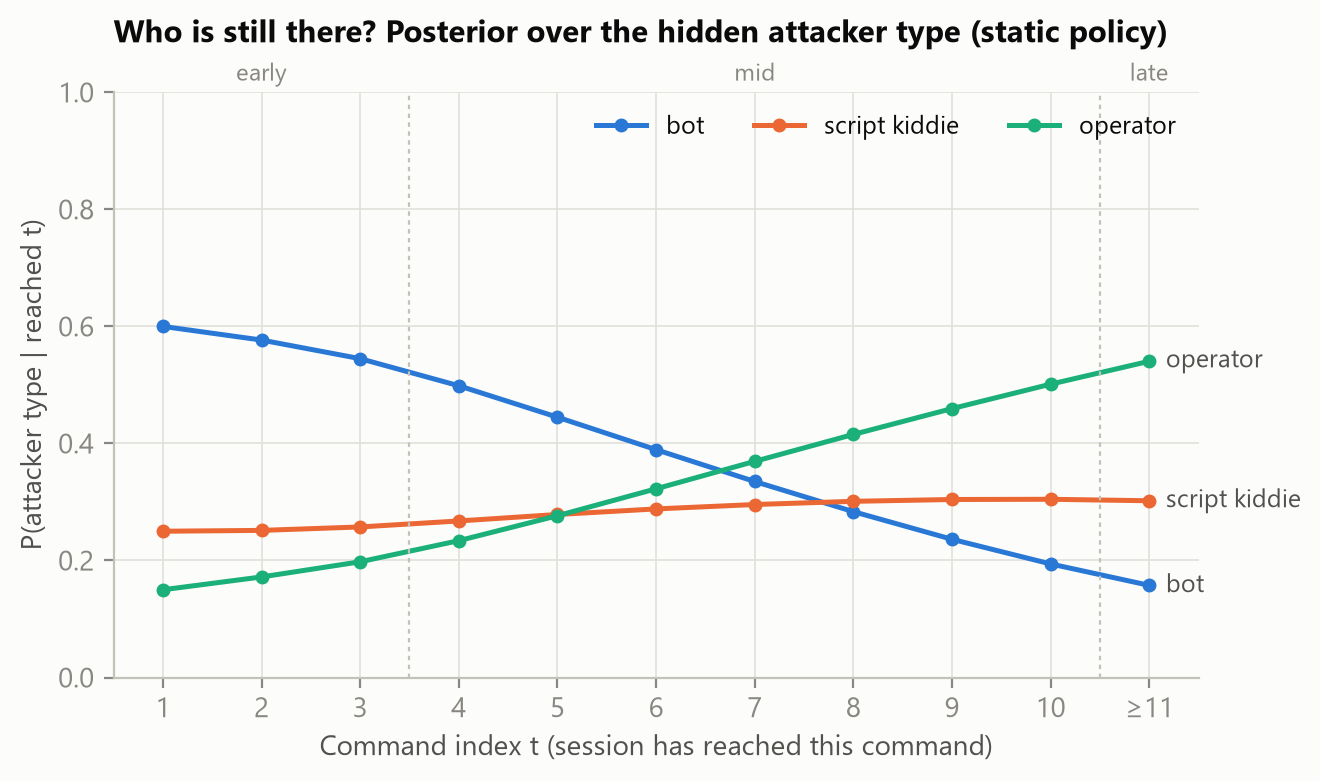
\includegraphics[width=0.85\textwidth]{fig_type_posterior.png}
\caption{Posterior probability of each attacker type given that the session has reached
command $t$ (static policy, balanced population).}
\label{fig:posterior}
\end{figure}

\section{Estimating the Model from Data}
\label{sec:fit}

Given the category sequences of captured sessions, the likelihood of a chain with initial
distribution $\mu$, transition matrix $P$ and exit probabilities $e$ is
\[
L = \prod_{\text{sessions}} \mu(c_1) \prod_{i=1}^{n-1} \big(1-e(c_i)\big) P(c_i, c_{i+1}) \cdot e(c_n).
\]
The likelihood factorises over $\mu$, over each row of $P$, and over each $e(c)$, and each factor
is a multinomial or Bernoulli likelihood. The maximiser is therefore the normalised counts:
\[
\hat\mu(c) = \frac{\#\text{starts at } c}{\#\text{sessions}}, \quad
\hat P(c,c') = \frac{\#(c \to c')}{\#(c \to \cdot)}, \quad
\hat e(c) = \frac{\#\text{ends at } c}{\#\text{visits to } c}.
\]
Laplace smoothing adds a pseudo-count to each transition. Fitted to sessions served by the
static policy, these estimates describe the attackers' own behaviour. Reaction multipliers can
be estimated only from sessions in which different actions were taken, which the live learner's
exploration provides.

\chapter{Implementation}
\label{ch:impl}

The system is implemented in Python 3.12 as four packages (\code{honeypot}, \code{pipeline},
\code{dashboard}, \code{simulator}) and deployed as five containers. Table~\ref{tab:loc}
summarises its size.

\begin{table}[H]
\centering
\begin{tabular}{@{}lrrr@{}}
\toprule
\textbf{Package} & \textbf{Source lines} & \textbf{Test lines} & \textbf{Tests} \\
\midrule
\code{honeypot} & 3{,}344 & 444 & 69 \\
\code{pipeline} & 375 & 191 & 12 \\
\code{dashboard} (+514 lines of templates, CSS, JS) & 328 & 112 & 20 \\
\code{simulator} & 879 & 101 & 10 \\
\midrule
Total & 4{,}926 & 848 & 111 \\
\bottomrule
\end{tabular}
\caption{Implementation size.}
\label{tab:loc}
\end{table}

\section{The Honeypot}

\subsection{SSH Server and Login Policy}

The server is built on AsyncSSH~\cite{asyncssh}. It advertises the version string of the
OpenSSH build that Ubuntu~22.04 ships,
\code{OpenSSH\_8.9p1\ Ubuntu-3ubuntu0.4}, and presents
both RSA and Ed25519 host keys. The keys are generated once and kept in a volume, so the
server's fingerprint is stable across restarts; a changing fingerprint is a honeypot tell.

Accepting every password on the first try is another well-known tell. For each source IP the
server therefore draws a threshold $N \sim U\{1,\dots,3\}$ and accepts the $N$-th attempt. Every
attempt (username, password, attempt number, outcome) becomes a \code{login\_attempt} event.

\subsection{Fake Filesystem}
\label{sec:fs}

Each session receives its own \code{FakeFileSystem}, an in-memory tree of nodes with
permissions, owners and timestamps. It is generated procedurally from a seed and discarded at
disconnect. It reproduces an Ubuntu~22.04 web/database server:
\begin{itemize}
  \item a standard root hierarchy and \code{/etc} (\code{passwd}, \code{shadow}, \code{group},
    \code{os-release}, \code{sshd\_config}, \code{crontab}, \code{nginx}, \code{mysql});
  \item \code{/proc} entries (\code{cpuinfo}, \code{meminfo}, \code{version}; \code{uptime} is computed live);
  \item lived-in content: a 60-line \code{auth.log} of failed logins, \code{syslog}, a nightly
    backup script and its log, \code{.bash\_history} for three users, binaries of realistic
    sizes in \code{/usr/bin}, and timestamps scattered over the past year;
  \item Unix permissions: a non-root user cannot read \code{/etc/shadow} or list \code{/root}.
\end{itemize}

\act{fake} calls \code{plant\_decoys()}, which idempotently adds honeytoken files and extends
\code{.bash\_history} with commands that point to them:
\begin{itemize}
  \item \code{/root/backup\_credentials.txt} and \code{/root/.my.cnf};
  \item \code{/home/deploy/.env};
  \item \code{/var/www/html/wp-config.php}.
\end{itemize}
To keep the repository free of anything resembling a real secret, every decoy value is a
visible placeholder such as \code{<decoy:mysql-root>}. The experiments measure \emph{whether}
attackers read decoys, which does not depend on how convincing the values look.

\subsection{Shell Emulator}

\code{Shell} parses each input line into statements separated by \code{;}, \code{\&\&},
\code{||} and \code{\&}. Exit status is tracked so that \code{false || echo x} and
\code{a \&\& b} behave as in Bash. It also handles quoting, pipelines, \code{>} and \code{>>}
redirection into the fake filesystem, \code{\$VAR} expansion and \code{VAR=value} assignments.
Paths such as \code{./x.sh} are resolved in the fake filesystem. A file with a shebang that
has been made executable has its lines interpreted, so the common
\code{wget \dots; chmod +x \dots; ./\dots} sequence works end to end, while a downloaded
``binary'' runs silently as a dropper would expect.

Command handlers are plain functions registered by a decorator into a table of 206 command
names, grouped into file and text commands, system and identity commands, and network
commands. A handler receives the shell, the arguments and any piped input, and returns text.
Unknown commands produce Bash's \code{command not found}. An exception inside any handler is
caught and yields empty output, so an emulation bug can never end a session.

\begin{lstlisting}[language=Python, caption={A command handler (simplified).}]
@command("whoami")
def whoami(sh, args, stdin=None):
    return sh.user + "\n"

@command("crontab")
def crontab(sh, args, stdin=None):
    if "-l" in args:
        node = sh.fs.get(f"/var/spool/cron/crontabs/{sh.user}")
        return node.content if node else f"no crontab for {sh.user}\n"
    # `crontab -` installs what was piped in, into the FAKE filesystem
    sh.fs.mkdir("/var/spool/cron/crontabs", parents=True, owner="root")
    sh.fs.write(f"/var/spool/cron/crontabs/{sh.user}", stdin or "")
    return ""
\end{lstlisting}

\subsection{Session Runner and the RL Loop}

\code{SessionRunner} owns one session. It prints the Ubuntu login banner and then loops:
read a line, classify it, form the state, ask the policy for an action, execute the line in
the emulator (with decoys if the action is \act{fake}), and deliver the output according to
the action. \act{delay} waits 1--4\,s. \act{tarpit} waits 4--7\,s and then writes 8-byte chunks
with pauses. \act{block} closes the channel. The reward for the previous command is computed and
the deferred TD update applied as soon as the next command arrives. At the end of the session
the terminal update is applied, $\varepsilon$ is decayed, and the Q-table is checkpointed
atomically (written to a temporary file and renamed).

All policies (Q-learning, SARSA, bandit, static, random) implement one interface:
\code{choose(state)}, \code{update(s, a, r, s', a')} and \code{end\_episode()}. The
\emph{same} classes run inside the honeypot and inside the simulator, together with the same
\code{compute\_reward} function, so simulation results apply to the deployed code.

\subsection{Event Emitter}

Events must reach Redis without ever slowing down or breaking a session (NFR2, NFR3). The
first implementation awaited \code{XADD} inline. Chapter~\ref{ch:testing} shows that this made
the honeypot disconnect every attacker while Redis was down. The final emitter uses
\emph{store-and-forward}. \code{emit()} serialises the event into a bounded in-memory queue
(50{,}000 events) and returns immediately. A background task forwards the queue to Redis in
order, retrying with exponential backoff (0.5\,s up to 30\,s) during outages. If an outage
outlasts the buffer, the oldest events are dropped and counted, never silently.

\section{The Pipeline}

The pipeline is a Redis Streams consumer in group \code{pipeline}. For each message it parses
the JSON, looks up the source IP's location (cached), applies the event to PostgreSQL in one
transaction, and only then acknowledges it (\code{XACK}). This gives at-least-once delivery.
Every write is idempotent, so redelivery is harmless:
\begin{itemize}
  \item attackers are upserted with \code{INSERT \dots{} ON CONFLICT (src\_ip) DO UPDATE},
    and their counters are incremented within the same statement;
  \item commands are inserted with \code{ON CONFLICT (session\_id, seq) DO NOTHING}, and the
    session's command count is incremented only if a row was actually inserted;
  \item a command that arrives before its \code{session\_start} creates a placeholder session row
    so that the foreign key holds.
\end{itemize}
On start-up the consumer first reclaims messages left pending by dead consumers
(\code{XAUTOCLAIM}) and replays its own pending messages, and only then reads new ones. Malformed
messages and those that fail with non-transient database errors are copied to a dead-letter
stream and acknowledged. Transient errors (connection lost) are retried with backoff. GeoIP
uses MaxMind GeoLite2~\cite{maxmind} when the database file is present; otherwise loopback
and private ranges are labelled and public addresses are left unknown.

\section{The Dashboard}

The dashboard is a read-only FastAPI~\cite{fastapi} application with Jinja2 templates and charts
rendered server-side as SVG and CSS, with no JavaScript chart library. It has five views
(Figures~\ref{fig:shot-overview}--\ref{fig:shot-rl}):
\begin{itemize}
  \item \textbf{Overview:} live counters refreshed every 10\,s from a JSON endpoint; sessions per
    hour; top usernames, passwords, commands and countries; the category mix and the agent's
    action mix.
  \item \textbf{Sessions and session detail:} filterable list; per-session metadata, an animated
    terminal replay of the commands, and a timeline showing, for each command, its category,
    phase, chosen action, reward, whether the attacker continued, and the greedy action before
    the decision.
  \item \textbf{Attackers:} per-IP profile with login attempts, behaviour mix and sessions.
  \item \textbf{RL agent:} learning curves, action mix over time, and the Q-table as a heatmap
    reconstructed from the \code{q\_after} values stored with each update.
\end{itemize}

Every username, password and command shown in the dashboard was typed by an attacker, which
makes the dashboard itself an attack surface: stored cross-site scripting against the analyst.
All such text is rendered through Jinja2 with autoescaping, and data passed to JavaScript goes
through \code{tojson}. The page has no inline scripts, and a Content-Security-Policy restricts
scripts to the same origin. A test injects \code{<script>} payloads as a username, password
and command and asserts that they never appear unescaped. When PostgreSQL is unavailable the
dashboard returns a 503 page that explains that capture continues.

\begin{figure}[H]
\centering
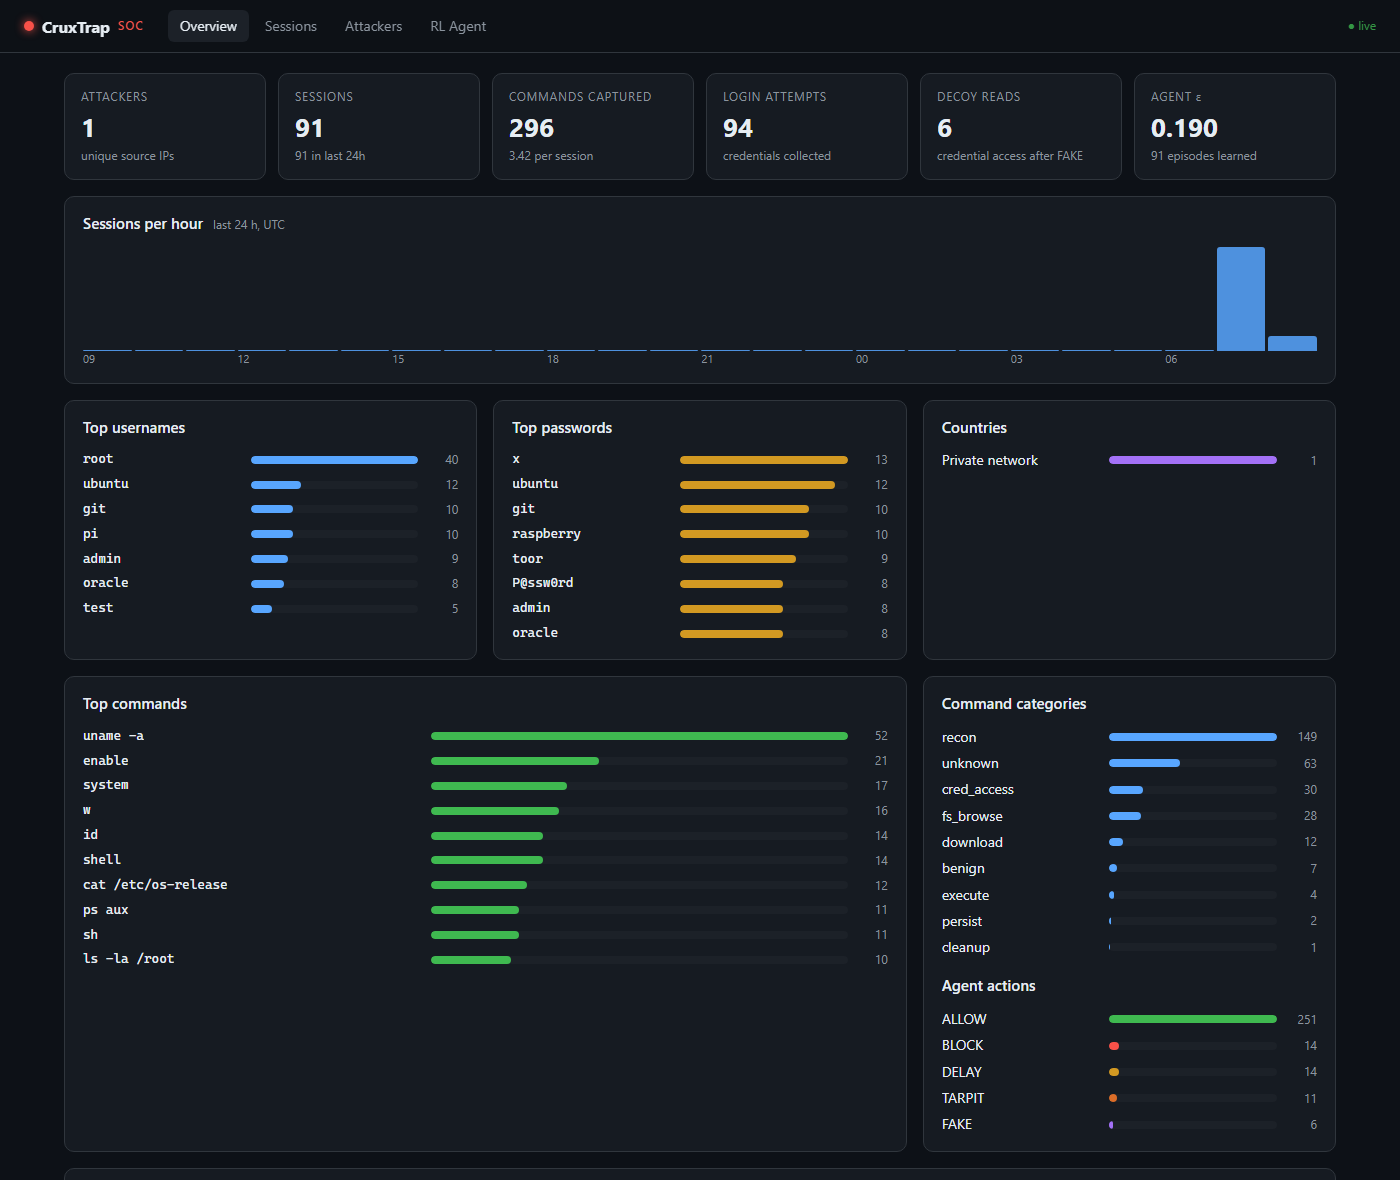
\includegraphics[width=\textwidth]{shot_overview.png}
\caption{Dashboard overview (lab-generated traffic).}
\label{fig:shot-overview}
\end{figure}

\begin{figure}[H]
\centering
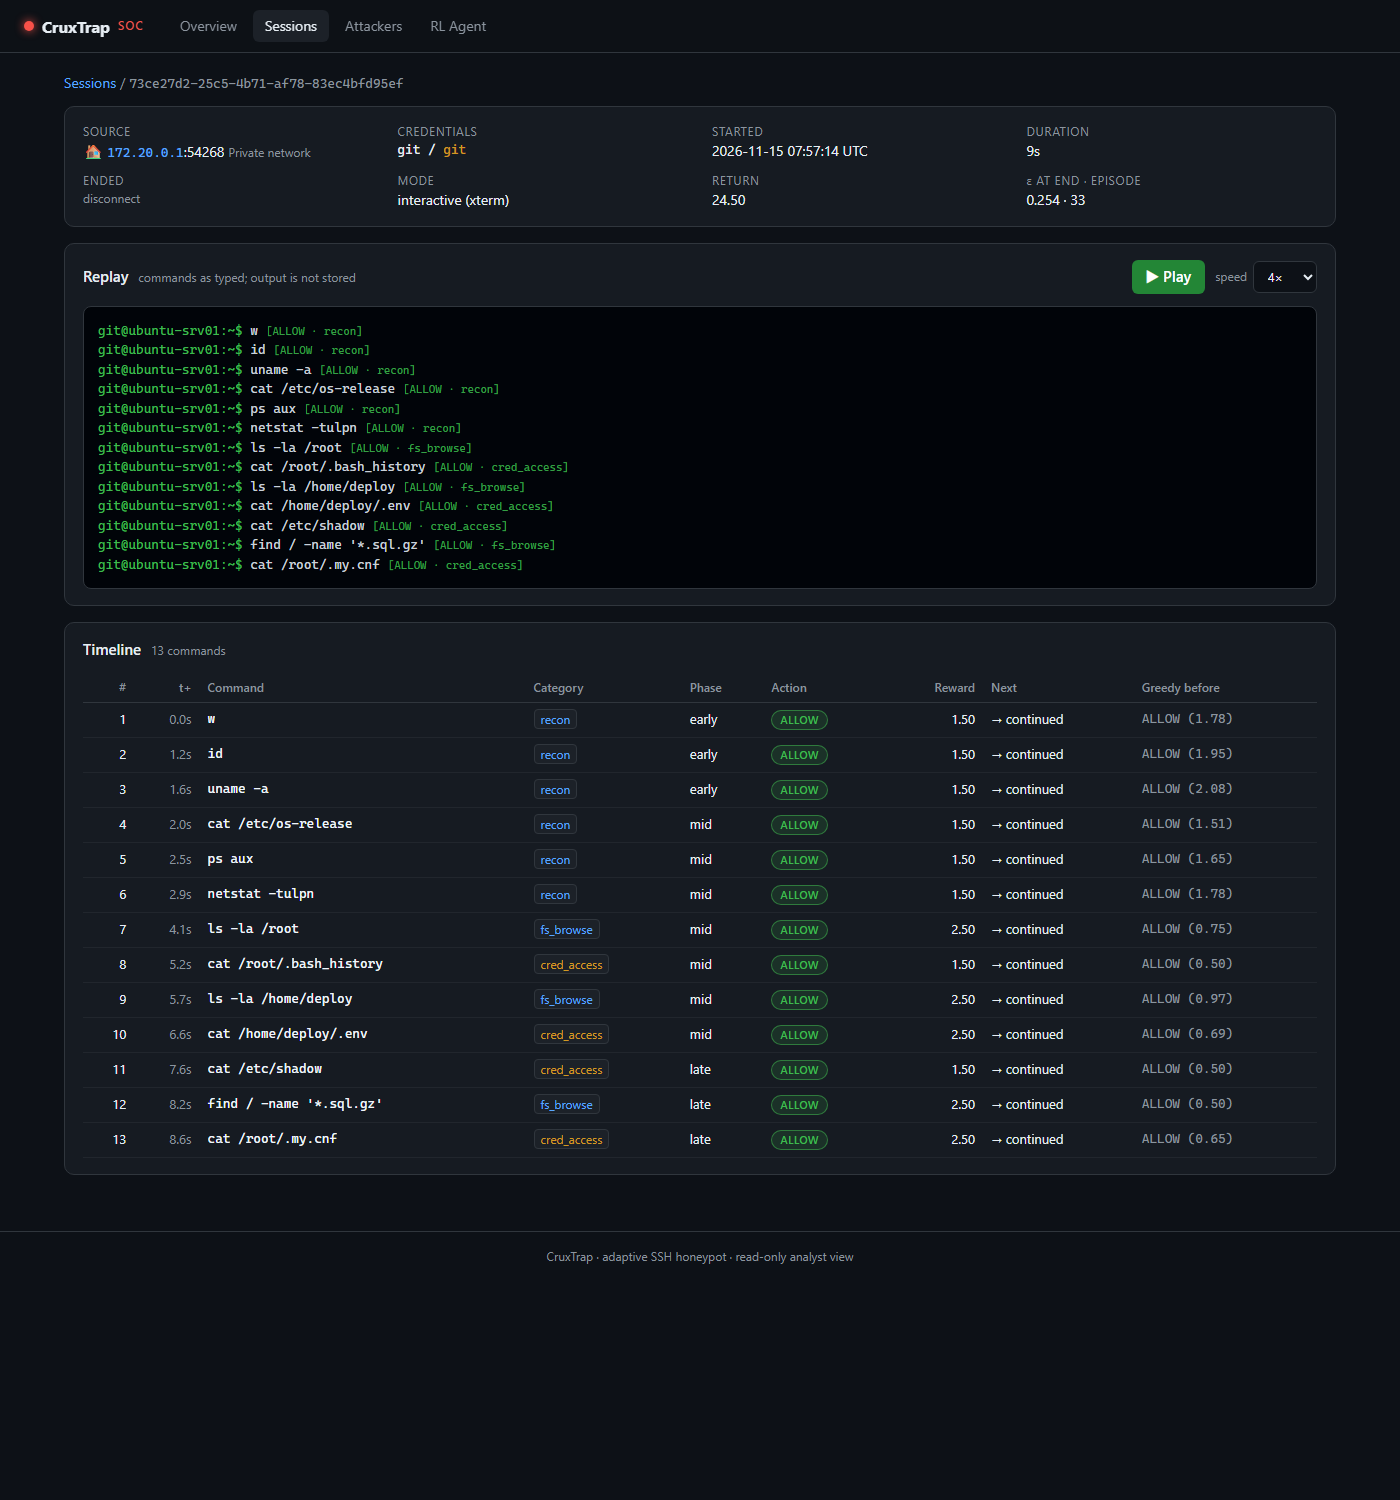
\includegraphics[width=\textwidth]{shot_session.png}
\caption{Session detail: terminal replay and per-command timeline with the agent's decisions.}
\label{fig:shot-session}
\end{figure}

\begin{figure}[H]
\centering
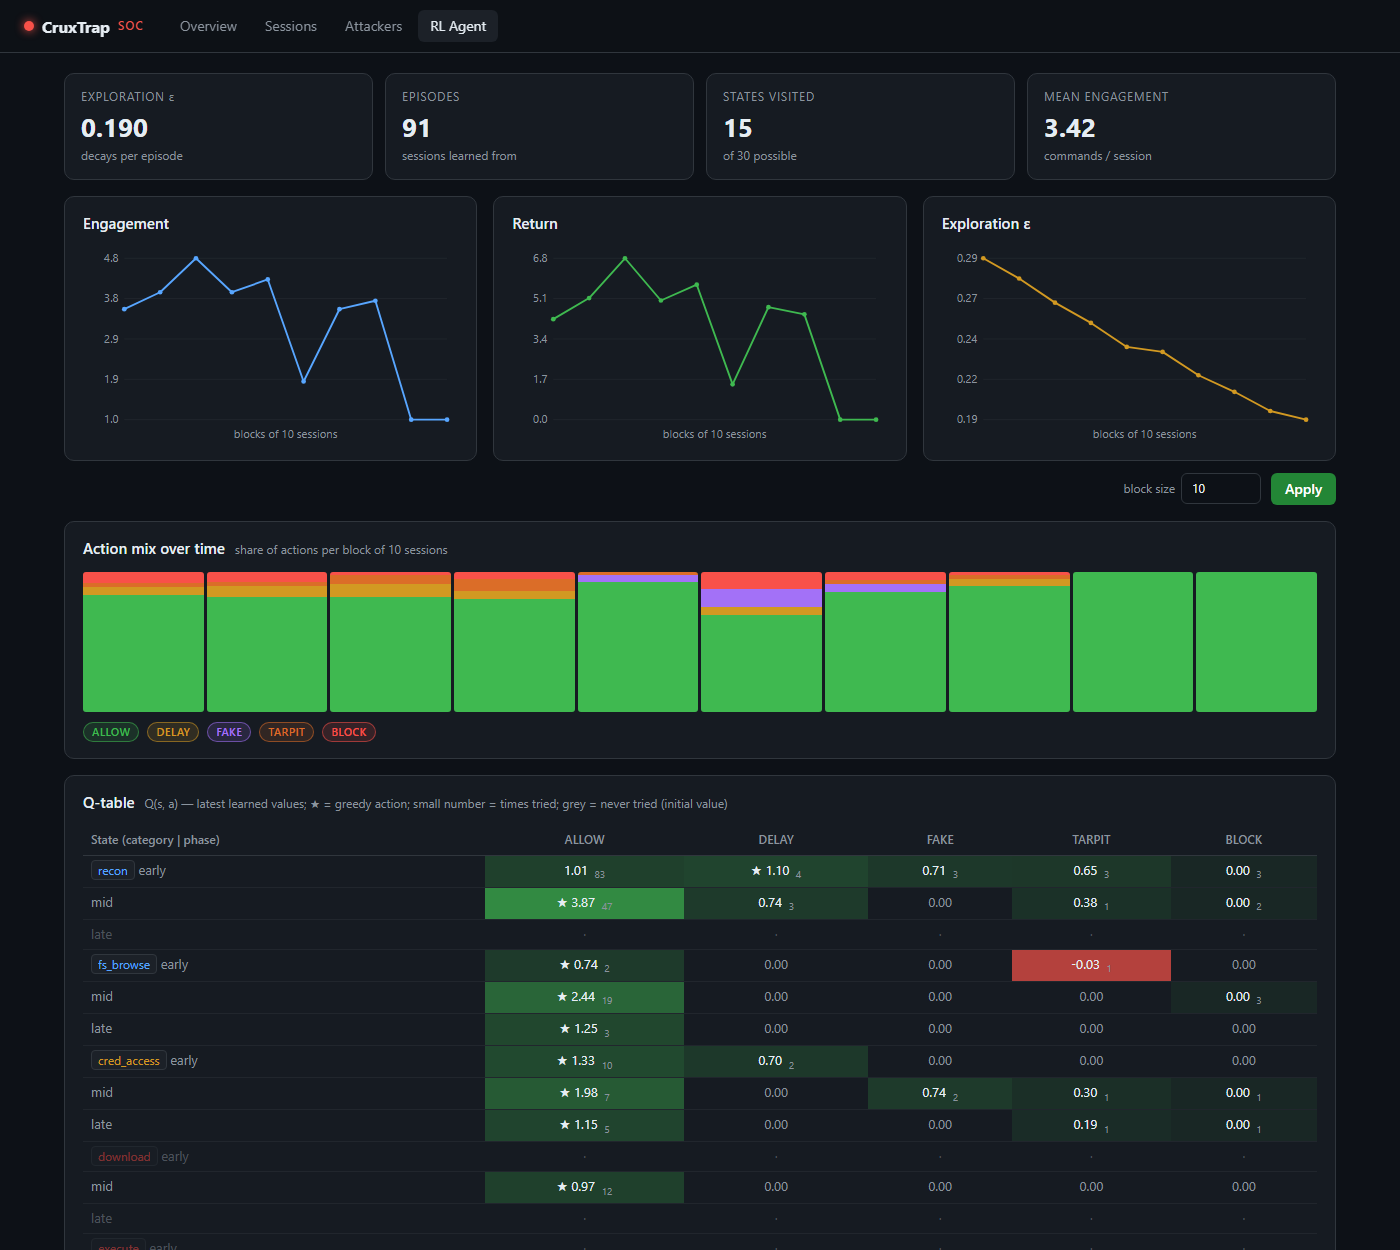
\includegraphics[width=\textwidth]{shot_rl.png}
\caption{RL view: learning curves, action mix over time and the Q-table heatmap.}
\label{fig:shot-rl}
\end{figure}

\section{Deployment}

Each Python service has its own image based on \code{python:3.12-slim} and runs as an
unprivileged user (UID 10001). Docker Compose defines the five services, their health checks,
start-up order (dependent services wait for healthy dependencies), three named volumes
(database, Redis append-only file, and honeypot keys plus Q-table), and two networks
(Figure~\ref{fig:arch}). Every published port binds to \code{127.0.0.1} by default. A real
deployment exposes only the honeypot, typically on port 22 after moving the host's own SSH
daemon. Table~\ref{tab:hardening} lists the hardening of the honeypot container.

\begin{table}[H]
\centering
\small
\begin{tabularx}{\textwidth}{@{}lX@{}}
\toprule
\textbf{Layer} & \textbf{Measure} \\
\midrule
Application & Emulation only: no \code{exec}, \code{subprocess} or shell anywhere in the command path \\
Process & Non-root UID 10001; effective capability set empty (\code{cap\_drop: ALL}); \code{no-new-privileges} \\
Filesystem & Read-only root filesystem; 16\,MB \code{tmpfs} at \code{/tmp} \\
Resources & 256 processes, 512\,MB memory, 1 CPU \\
Network & \code{ingest} network only: Redis reachable, PostgreSQL not resolvable \\
Health check & Reads \code{/proc/net/tcp} for the listening socket instead of connecting, so health probes are not recorded as attackers \\
\bottomrule
\end{tabularx}
\caption{Hardening of the internet-facing container.}
\label{tab:hardening}
\end{table}

\paragraph{Source addresses.} On Docker Desktop (Windows and macOS), published ports pass
through a user-space proxy, and the honeypot sees every client as the Docker gateway address.
On a Linux host, connections from the Internet are forwarded by iptables DNAT and keep their
real source address. The honeypot must therefore be deployed on Linux, or with host
networking, for the source-IP telemetry to be meaningful.

\chapter{Testing and Verification}
\label{ch:testing}

Testing had three layers: automated tests that run in four seconds to two minutes, security
verification of the running containers, and failure experiments on the live stack. The second
and third layers found four defects that the automated tests had missed (Section~\ref{sec:bugs}).

\section{Automated Tests}

The 111 tests run with \code{python -m pytest}. Pipeline and dashboard tests use a separate
\code{cruxtrap\_test} database and a unique stream name per test, so they never touch collected
data, and they are skipped if Redis or PostgreSQL is not running.

\begin{longtable}{@{}p{4.2cm}cp{8.6cm}@{}}
\toprule
\textbf{Test module} & \textbf{Tests} & \textbf{What is verified} \\
\midrule
\endhead
\code{test\_classify} & 25 & Category of 22 representative commands, including \code{sudo}-prefixed and chained lines; phase boundaries. \\
\code{test\_fakefs} & 8 & Ubuntu layout; path resolution (\code{..}, \code{\textasciitilde}); write/append/remove; permissions for non-root users; isolation between sessions; decoys are placeholders and idempotent. \\
\code{test\_shell} & 15 & Prompt and \code{cd}; recon output; \code{ls} variants; chaining, pipes, \code{||}; redirection and script execution; the download-and-execute flow; persistence (\code{authorized\_keys}, \code{crontab}, \code{useradd}); non-root restrictions; decoy mode; 15 malformed inputs never raise. \\
\code{test\_policies} & 12 & Reward function; justified-block bonus; static and warm-start behaviour; Q-learning learns the better action in a toy problem; SARSA and bandit updates; $\varepsilon$ decay; step-size schedules; checkpoint round-trip. \\
\code{test\_emitter} & 4 & Ordered forwarding; \code{emit} never blocks on a slow Redis; an outage buffers events and then delivers them all, in order; the bounded buffer drops the oldest events. \\
\code{test\_server} & 5 & A real SSH client against the server: \code{exec} round trip; an interactive session that produces the expected categories, TD updates and checkpoint; \act{block} closes the connection; \act{fake}, \act{tarpit} and \act{delay} still answer; the $N$-th-attempt login policy. \\
\code{test\_pipeline} & 12 & A full session lands in all four tables; idempotent redelivery; command before session start; dead-lettering; replay after a crash; claiming orphans of a dead consumer; an idle blocking read; Redis outage; group recreation; \textbf{SSH client $\rightarrow$ honeypot $\rightarrow$ Redis $\rightarrow$ pipeline $\rightarrow$ PostgreSQL}. \\
\code{test\_dashboard} & 20 & Every page renders with and without data; session replay; JSON statistics; \textbf{injected \code{<script>} never rendered}; security headers; 404 handling; 503 on database outage. \\
\code{test\_simulator} & 10 & Model rows are probability distributions; \textbf{Monte-Carlo means within 4 standard errors of the exact values} (static, random and a trained policy, 30{,}000 episodes each); benchmark ordering oracle $\ge$ best observable $\ge$ static; Bellman residual of value iteration $< 10^{-8}$; MLE recovers a known chain; type posterior. \\
\bottomrule
\caption{Automated test suite.}
\label{tab:tests}
\end{longtable}

\section{Security Verification}

The properties claimed in Table~\ref{tab:hardening} were checked on the running containers:

\begin{table}[H]
\centering
\small
\begin{tabular}{@{}ll@{}}
\toprule
\textbf{Check (inside the honeypot container)} & \textbf{Observed} \\
\midrule
\code{id} & \code{uid=10001(cruxtrap) gid=10001(cruxtrap)} \\
\code{touch /app/x} & \code{Read-only file system} \\
\code{CapEff} in \code{/proc/self/status} & \code{0000000000000000} \\
connect to \code{postgres:5432} & \code{Name or service not known} \\
connect to \code{redis:6379} & succeeds \\
Host listeners on 2222, 6379, 8000, 55432 & all bound to \code{127.0.0.1} \\
\bottomrule
\end{tabular}
\caption{Security verification on the live deployment.}
\label{tab:secverify}
\end{table}

\section{Failure Experiments}

Each component downstream of the honeypot was stopped in turn. SSH sessions were opened during
the outage, and the component was then restarted.

\begin{table}[H]
\centering
\small
\begin{tabularx}{\textwidth}{@{}lccX@{}}
\toprule
\textbf{Outage} & \textbf{Attackers served} & \textbf{Recovered} & \textbf{Observation} \\
\midrule
Redis & yes & all & Honeypot logged \emph{buffering events}, then \emph{forwarding 23 buffered events} \\
PostgreSQL & 4/4 & 4/4 & Events waited in the stream; dashboard returned 503; pipeline did not restart \\
Pipeline & 4/4 & 4/4 & Resumed from its consumer-group position \\
None (idle 40\,s) & -- & -- & 0 restarts (regression check for defect D2) \\
\bottomrule
\end{tabularx}
\caption{Behaviour under component failure. After all scenarios there were no dead-lettered events and no command without a recorded reward.}
\label{tab:outages}
\end{table}

\paragraph{Limitation.} The emitter's buffer is held in memory, so events emitted during a
Redis outage are lost if the honeypot process also crashes before Redis returns. A disk-backed
spool would close this gap.

\section{Defects Found by Running the System}
\label{sec:bugs}

\begin{longtable}{@{}p{0.6cm}p{4.2cm}p{4.6cm}p{4.2cm}@{}}
\toprule
& \textbf{Symptom} & \textbf{Cause} & \textbf{Fix} \\
\midrule
\endhead
D1 & Pipeline crashed on the first scanner that disconnected without logging in & The attacker upsert with no counters to increment generated invalid SQL & Correct SQL generation; non-transient database errors are dead-lettered instead of crashing \\
D2 & Pipeline container restarted every few seconds when idle & The client socket timeout was shorter than the \code{XREADGROUP BLOCK} window, and the code caught Python's \code{ConnectionError} rather than redis-py's exceptions & Socket timeout longer than the block window; catch \code{RedisError}; recreate the group on \code{NOGROUP} \\
D3 & Every attacker was disconnected while Redis was down & The emitter awaited \code{XADD} inside SSH authentication & Store-and-forward emitter \\
D4 & Dashboard charts were blank & The CSP \code{style-src 'self'} blocked the inline style attributes that set bar widths & Allow inline styles only; scripts remain same-origin only \\
D5 & Exact solver about 100$\times$ slower than expected & Multi-threaded OpenBLAS overhead on $330 \times 330$ solves & Pin BLAS to one thread; parallelise across processes instead \\
\bottomrule
\caption{Defects found by running the system rather than by unit tests.}
\label{tab:bugs}
\end{longtable}

D1--D3 share a lesson: unit tests exercised each component in its steady state, but each defect
appeared only at a boundary (an unauthenticated client, an idle period, a dependency outage).
D3 is the most significant, because it contradicted the architecture's central claim that
capture does not depend on downstream components. Each of D1--D3 now has a regression test.

\chapter{Results and Evaluation}
\label{ch:results}

This chapter answers RQ1 and RQ2 using the attacker model and the exact evaluation of
Chapter~\ref{ch:formulation}. Every number in it is reproduced, with fixed seeds, by the
command \code{python -m simulator.experiments}, which takes about one minute on eight cores.

\section{Experimental Protocol}

\begin{itemize}
  \item \textbf{Policies:} Q-learning and SARSA on the 30-state observation; an $\varepsilon$-greedy
    bandit that ignores the state; the static honeypot (always \act{allow}); a uniformly random policy.
  \item \textbf{Hyper-parameters:} $\gamma = 0.9$; $\varepsilon$ from 0.3 decaying by a factor
    of 0.995 per episode to a floor of 0.05; $\alpha_n = n^{-0.7}$ per state--action pair.
  \item \textbf{Main experiment:} balanced population, 20 seeds $\times$ 20{,}000 episodes per
    learner. At the end, each run's greedy policy is evaluated \emph{exactly}. The spread across
    seeds therefore reflects learning alone, not evaluation noise.
  \item \textbf{Statistics:} 95\% Student-$t$ confidence intervals over seeds; a one-sided
    one-sample $t$-test of Q-learning against the deterministic static value; Welch's $t$-test
    between Q-learning and SARSA.
  \item \textbf{Seed hygiene:} the step-size schedule was chosen in a pilot on disjoint seeds
    and fixed before the reported runs. Main, sensitivity, ablation and diagnostic runs all use
    disjoint seed ranges.
\end{itemize}

\paragraph{Validation of the exact evaluator.} For the policy learned by seed~0, 50{,}000
simulated episodes give a mean return of $5.442 \pm 0.043$ and $3.884 \pm 0.027$ commands. The
exact values are $5.464$ and $3.899$, both inside the intervals. The unit tests check the same
agreement for three further policies.

\section{RQ1: Learned versus Static Responses}

\begin{table}[H]
\centering
\begin{tabular}{@{}lccc@{}}
\toprule
\textbf{Policy} & \textbf{Return} & \textbf{Commands/session} & \textbf{Intel/session} \\
\midrule
Q-learning & $\mathbf{5.686 \pm 0.051}$ & $4.056 \pm 0.034$ & $9.91 \pm 0.10$ \\
SARSA & $\mathbf{5.702 \pm 0.026}$ & $4.064 \pm 0.018$ & $9.93 \pm 0.05$ \\
$\varepsilon$-greedy bandit & $5.503 \pm 0.021$ & $3.982 \pm 0.028$ & $9.58 \pm 0.03$ \\
Static (always \act{allow}) & $5.542$ & $4.034$ & $9.64$ \\
Random & $1.949$ & $2.015$ & $3.91$ \\
\midrule
Best observable policy & $5.783$ & $4.157$ & $10.22$ \\
Oracle (type observed) & $5.935$ & -- & -- \\
\bottomrule
\end{tabular}
\caption{Exact expected performance of the final greedy policies (mean $\pm$ 95\% CI over 20 seeds).}
\label{tab:main}
\end{table}

\begin{figure}[H]
\centering
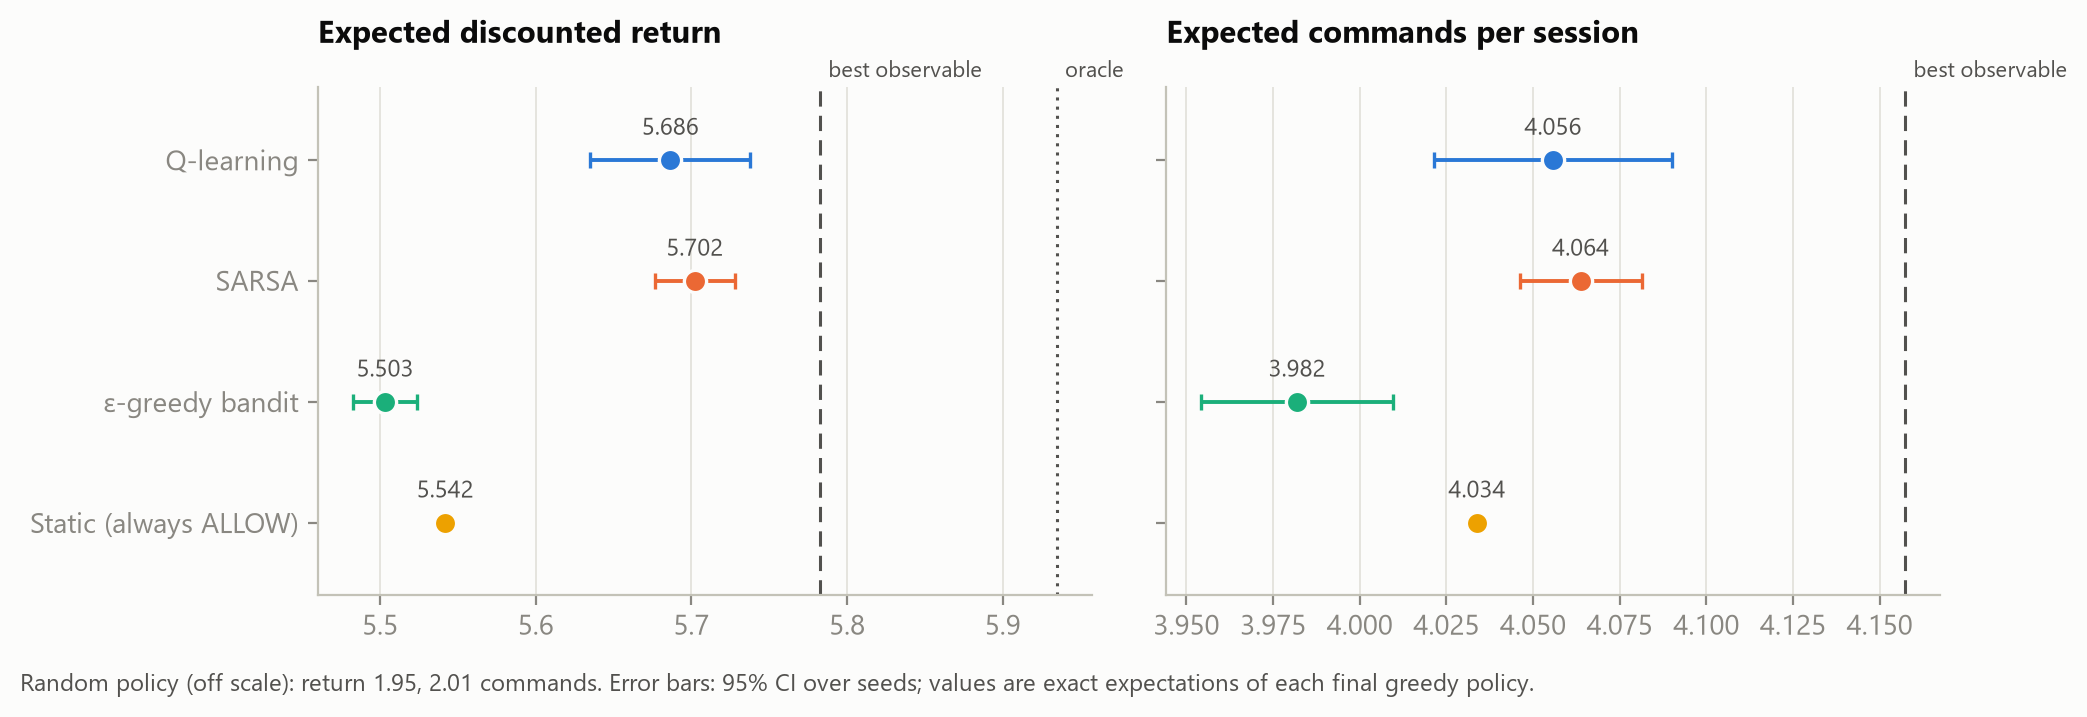
\includegraphics[width=\textwidth]{fig_final_performance.png}
\caption{Final greedy policies against the best observable policy and the oracle.}
\label{fig:final}
\end{figure}

\begin{enumerate}
  \item \textbf{Learning beats the static honeypot.} Q-learning's return exceeds static by
    2.6\% ($t = 5.88$, $p = 5.8 \times 10^{-6}$, $n = 20$). It recovers $60\% \pm 21\%$ of the
    gap between static and the best observable policy. Engagement rises by 0.5\% and captured
    intelligence by 2.8\%: the gain comes from \emph{which} sessions are prolonged, namely
    credential-hunting ones, more than from how many commands are seen.
  \item \textbf{Q-learning and SARSA are indistinguishable} (Welch $p = 0.57$).
  \item \textbf{State matters.} The bandit, which must pick one action for all situations,
    does \emph{worse} than static. No single action beats \act{allow} everywhere.
  \item \textbf{The remaining headroom needs information the honeypot lacks.} The oracle exceeds
    the best observable policy by a further 2.6\%, but only by knowing the attacker's type.
\end{enumerate}

\subsection{What the Agent Learns}

The best observable policy departs from \act{allow} in exactly one place: \textbf{\act{fake} on
credential access, in every phase}. Figure~\ref{fig:policymap} shows that Q-learning finds this
in every seed for the early and mid phases and in 80\% of seeds for the late phase. The policy
agrees with the best one in 68\% of states, yet achieves 60\% of its gain. Most disagreements
occur where actions are nearly equivalent (bots barely react) or in rarely visited states,
where a wrong choice costs almost nothing.

\begin{figure}[H]
\centering
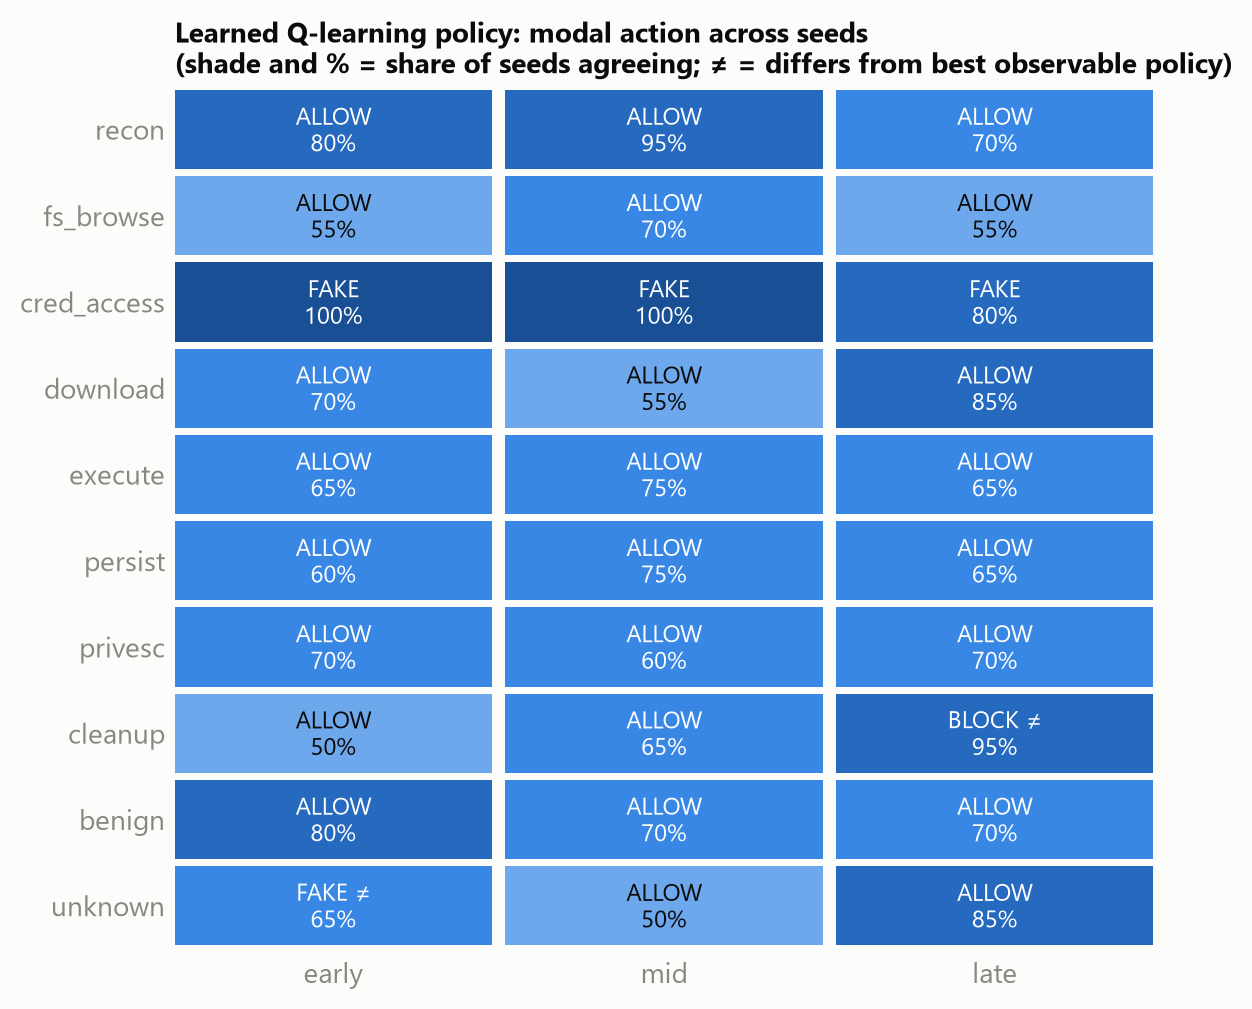
\includegraphics[width=0.78\textwidth]{fig_policy_map.png}
\caption{Modal action learned by Q-learning in each state across 20 seeds; the shading gives the share of seeds that agree.}
\label{fig:policymap}
\end{figure}

\subsection{Learning Dynamics and the Cost of Exploration}

\begin{figure}[H]
\centering
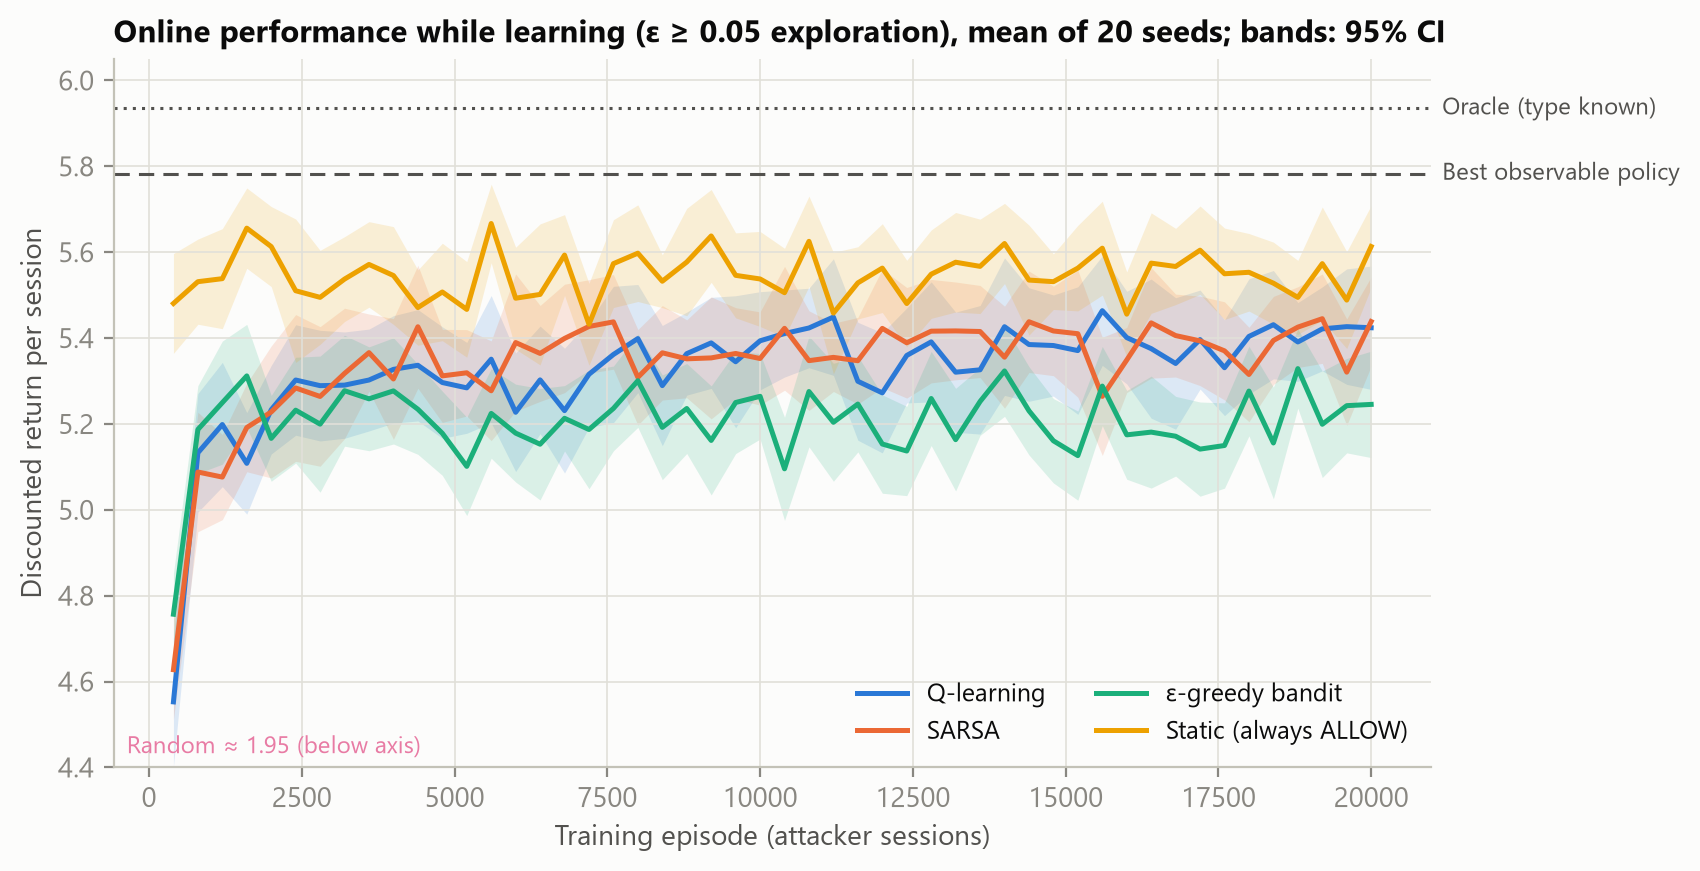
\includegraphics[width=\textwidth]{fig_learning_curves.png}
\caption{Online return during learning (block means of 400 episodes; bands are 95\% CIs over seeds).}
\label{fig:curves}
\end{figure}

Online performance includes exploration: with $\varepsilon \ge 0.05$, about one action in
twenty is random, and some of those are session-ending \act{block}s. During learning, all three
learners therefore stay \emph{below} the static honeypot (about 5.42 against 5.55 at the end),
even though the greedy policies they have learned are better than static. The exploration needed
to keep learning costs about as much as adaptation gains. In deployment, $\varepsilon$ should
therefore decay towards zero once the policy has settled. A GLIE schedule does this, as does
serving the greedy policy while learning off-policy from logged sessions.

\section{Step Size: a Negative Result Explained by Theory}

The first run used the constant step size $\alpha = 0.1$ from the original design. The learned
policies were \emph{worse} than the static honeypot: $5.343 \pm 0.154$ after 5{,}000 episodes,
better than static in only 2 of 10 seeds. The diagnosis follows Section~\ref{sec:learning}. With
constant $\alpha$, the noise in each estimate stays at about $0.23\sigma$. In the most visited
states, such as \code{recon|early}, the true differences between actions are of the same size,
because bots barely react to the response. The greedy choice is therefore decided by noise, and
half of the seeds chose a non-\act{allow} action there.

\begin{table}[H]
\centering
\begin{tabular}{@{}lcc@{}}
\toprule
\textbf{Step size} & \textbf{5{,}000 episodes} & \textbf{20{,}000 episodes} \\
\midrule
constant $\alpha = 0.1$ & $5.343 \pm 0.154$ \;(2/10) & $5.479 \pm 0.150$ \;(4/10) \\
$\alpha_n = n^{-0.6}$ & $5.662 \pm 0.080$ \;(9/10) & $5.618 \pm 0.138$ \;(7/10) \\
$\alpha_n = n^{-0.7}$ (main) & $5.608 \pm 0.155$ \;(8/10) & $\mathbf{5.710 \pm 0.043}$ \;(10/10) \\
$\alpha_n = n^{-0.85}$ & $5.610 \pm 0.092$ \;(7/10) & $5.676 \pm 0.067$ \;(8/10) \\
$\alpha_n = 1/n$ & $5.513 \pm 0.087$ \;(4/10) & $5.611 \pm 0.083$ \;(6/10) \\
\bottomrule
\end{tabular}
\caption{Step-size ablation (Q-learning, 10 seeds each). In parentheses: number of seeds whose final policy beats static (5.542).}
\label{tab:ablation}
\end{table}

\begin{figure}[H]
\centering
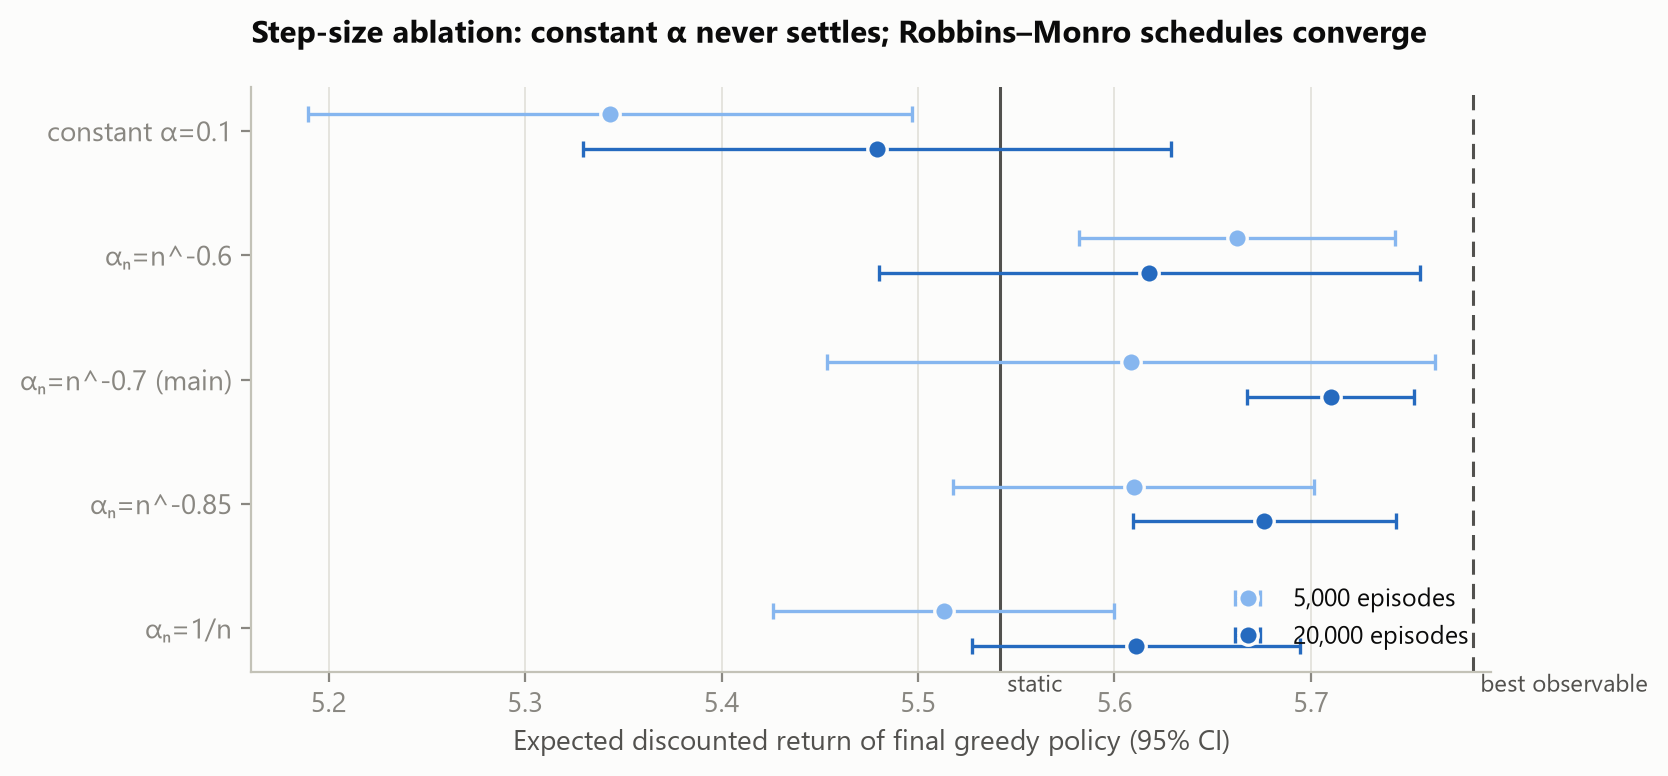
\includegraphics[width=0.92\textwidth]{fig_ablation_step_size.png}
\caption{Step-size ablation.}
\label{fig:ablation}
\end{figure}

The Robbins--Monro schedules all beat static. Among them, $1/n$ is the weakest. This agrees
with Even-Dar and Mansour~\cite{evendar2003rates}: with $1/n$, the early bootstrapped targets,
which are wrong, keep too much weight for too long. The differences among
$\omega \in \{0.6, 0.7, 0.85\}$ are not significant with 10 seeds. The robust conclusion is that
the step size must decay, and must decay more slowly than $1/n$.

\section{A Residual Bias}

In 95\% of runs Q-learning chooses \act{block} in \code{cleanup|late}, where the best observable
policy keeps \act{allow}. A diagnostic on fresh seeds found that the learned $Q(\act{allow})$
there is $1.18$ against a true $2.04$, while $Q(\act{block})$ is exact ($2.00$ against $2.00$).
Late states are rarely visited, so the values that \act{allow} bootstraps from are still near
their initial levels. \act{block}'s target is terminal and does not bootstrap. Once \act{block}
is greedy, \act{allow} receives only half as many updates (109 against 199), so the underestimate
persists. The cost is 0.0017 in return (0.03\%). Optimistic initial values or double
Q-learning~\cite{vanhasselt2010double} are standard remedies and are left as future work rather
than tuned on the reported seeds.

\section{RQ2: Sensitivity to Attackers and Objective}

\begin{table}[H]
\centering
\begin{tabular}{@{}llcccc@{}}
\toprule
\textbf{Mix} & \textbf{Objective} & \textbf{Static} & \textbf{Q-learning} & \textbf{Best obs.} & \textbf{Oracle} \\
\midrule
balanced & intel & 5.542 & $5.736 \pm 0.012$ & 5.783 & 5.935 \\
bot-heavy & intel & 5.133 & $5.159 \pm 0.039$ & 5.222 & 5.281 \\
human-heavy & intel & 6.273 & $6.600 \pm 0.060$ & 6.740 & 6.953 \\
balanced & attrition & 5.542 & $5.659 \pm 0.076$ & 5.783 & 5.937 \\
bot-heavy & attrition & 5.133 & $5.135 \pm 0.038$ & 5.222 & 5.282 \\
human-heavy & attrition & 6.273 & $6.634 \pm 0.055$ & 6.740 & 6.957 \\
\bottomrule
\end{tabular}
\caption{Sensitivity analysis (10 seeds per scenario). The attrition objective rewards attacker time consumed ($w_c = -0.05$).}
\label{tab:sens}
\end{table}

\begin{figure}[H]
\centering
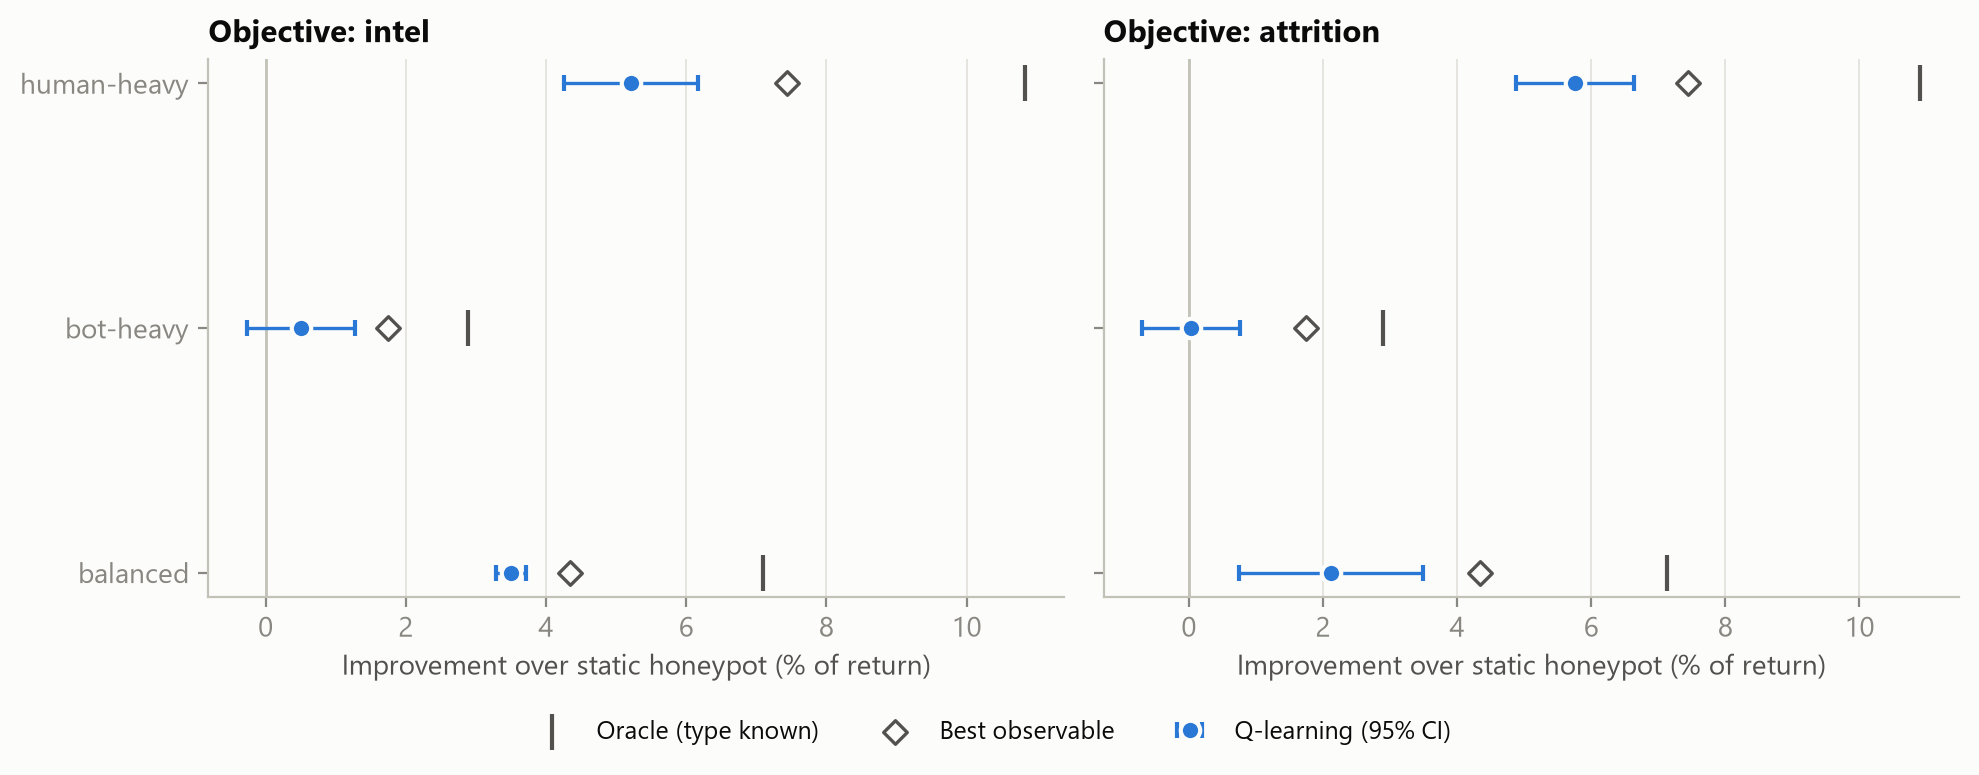
\includegraphics[width=\textwidth]{fig_sensitivity.png}
\caption{Improvement over the static honeypot by population and objective.}
\label{fig:sens}
\end{figure}

\begin{itemize}
  \item \textbf{Adaptation pays in proportion to how adaptive the attackers are.} The gain over
    static is $+0.5\%$ against bot-heavy traffic (not significant), $+3.5\%$ against the balanced
    mix and $+5.2\%$ against human-heavy traffic. Against scripted bots, a static honeypot is
    already near-optimal.
  \item \textbf{The learned structure is stable.} \act{fake} on credential access appears in every
    scenario. With many bots, the best policy also uses \act{fake} on file browsing. Under the
    attrition objective it uses \act{delay} on late cleanup, slowing down sessions that are
    about to end at no cost in intelligence.
  \item \textbf{\act{tarpit} is never chosen}, even when wasting attacker time is rewarded. Under
    this model, the sessions it would end are worth more than the time it would waste.
\end{itemize}

\section{Threats to Validity}

\begin{enumerate}
  \item \textbf{Model dependence.} Effect sizes depend on the assumed reaction multipliers. The
    qualitative conclusions hold in all six scenarios: static is near-optimal against bots,
    \act{fake} on credential access is the robust deviation, and the step size must decay.
    Fitting the model to captured sessions (Section~\ref{sec:fit}) is the way to tighten them.
  \item \textbf{Abstraction.} The simulator generates command categories, not command strings,
    so misclassification of real input is not modelled.
  \item \textbf{Stationarity.} Real attacker populations drift; the experiments use a fixed mixture.
  \item \textbf{Reward design.} Conclusions are also reported in reward-independent units
    (commands and intelligence per session).
  \item \textbf{Benchmark optimality.} The best observable policy is a strong local optimum of an
    NP-hard problem, not a proven optimum.
\end{enumerate}

\chapter{Conclusion and Future Work}
\label{ch:conclusion}

\section{Conclusion}

This project set out to test whether an SSH honeypot that chooses its responses can capture more
attacker behaviour than one that does not, and to measure the benefit rigorously.

We built \textbf{CruxTrap}, a complete five-service system. It consists of a safe
medium-interaction honeypot with a per-session emulated Ubuntu server and over 200 emulated
command names, an online reinforcement-learning response policy, an at-least-once event pipeline
through Redis Streams into PostgreSQL, and an analyst dashboard with session replay and a view of
the learned policy. The system is containerised with defence-in-depth hardening. Its key safety
and availability properties were verified on the running deployment: an unprivileged, read-only,
capability-free honeypot that cannot reach the database, and continued attack capture through
Redis, pipeline and database outages.

We formalised the honeypot's problem as an MDP whose reward measures captured intelligence, and
identified that it is partially observable because the attacker's type is hidden. For evaluation
we built a generative attacker model and an \emph{exact} evaluator. The evaluator computes each
policy's expected return, engagement and intelligence by solving the Bellman equations on a
330-state augmented chain; it also gives an oracle upper bound and the best policy available to
the honeypot's own state.

The main findings are:
\begin{enumerate}
  \item Q-learning beats a static honeypot with high confidence ($5.686$ against $5.542$,
    $p = 5.8 \times 10^{-6}$) and recovers 60\% of the achievable improvement. It does this by
    discovering, without supervision, a single robust deception: serving decoy credentials to
    attackers who are searching for credentials.
  \item This holds only with a step size that satisfies the Robbins--Monro conditions. With the
    conventional constant learning rate the agent did worse than static, because the estimates
    never settle and noise decides the greedy action. An ablation confirmed the explanation.
  \item The benefit is modest and depends on the population: it is negligible against scripted
    bots and about 5\% against human-heavy traffic. Adaptation pays where attackers adapt.
  \item Exploration while live costs about as much as adaptation gains, so a deployment should
    reduce exploration once the policy has settled.
\end{enumerate}

The broader lesson is methodological. Deploying an adaptive honeypot and reporting that
attackers stayed longer does not establish that adaptation helped. A model with exact evaluation
makes it possible to ask how much better a policy is, compared with what is achievable, and
against whom.

\section{Future Work}

\begin{itemize}
  \item \textbf{Real-traffic study.} Deploy the honeypot on a Linux host with a public address.
    Fit the attacker model to sessions captured under the static policy, then compare the learned
    and static policies on live traffic with an interleaved (A/B) design.
  \item \textbf{Richer state.} Add the previous action, a short command history, or a belief over
    the attacker type estimated from inter-command timing. The posterior in
    Figure~\ref{fig:posterior} suggests that even a coarse type estimate is valuable. Beyond a few
    hundred states, linear function approximation or a small DQN becomes appropriate.
  \item \textbf{Exploration and bias.} Use GLIE schedules for deployment, optimistic
    initialisation or double Q-learning for the late-state bias, and off-policy evaluation from
    logged data.
  \item \textbf{Durability.} Use a disk-backed spool in the emitter so that events survive a
    simultaneous Redis outage and honeypot crash.
  \item \textbf{Capture.} Add SFTP/SCP file capture, sandboxed analysis of downloaded payloads, and
    threat-intelligence enrichment of indicators.
  \item \textbf{Operations.} Add dashboard authentication and HTTPS, alerting, SIEM export, and
    orchestration (for example Kubernetes) for multi-sensor deployments.
\end{itemize}


\clearpage
\phantomsection
\addcontentsline{toc}{chapter}{References}
\bibliographystyle{unsrt}
\bibliography{refs}

\appendix
\chapter{Running the System}
\label{app:run}

\section{Deployment}

\begin{lstlisting}[language=bash]
git clone https://github.com/mohd-kalam121/cruxtrap && cd cruxtrap
docker compose up -d --build          # all five services, localhost only
ssh -p 2222 root@127.0.0.1            # the honeypot (N-th password attempt succeeds)
# dashboard: http://127.0.0.1:8000

# Real deployment on a Linux host: expose only the honeypot, on port 22
HONEYPOT_BIND=0.0.0.0 HONEYPOT_PORT=22 docker compose up -d
\end{lstlisting}

\section{Reproducing the Results}

\begin{lstlisting}[language=bash]
python -m venv .venv && . .venv/bin/activate
pip install -r honeypot/requirements.txt -r simulator/requirements.txt
python -m simulator.experiments       # ~1 min; writes docs/results and docs/figures
python -m pytest                      # 111 tests (needs Redis/PostgreSQL for 32 of them)
\end{lstlisting}

\section{Configuration}

\begin{longtable}{@{}p{5.2cm}p{2.6cm}p{6cm}@{}}
\toprule
\textbf{Variable} & \textbf{Default} & \textbf{Meaning} \\
\midrule
\endhead
\code{HONEYPOT\_BIND}, \code{HONEYPOT\_PORT} & 127.0.0.1, 2222 & Host address and port of the honeypot \\
\code{HONEYPOT\_HOSTNAME} & ubuntu-srv01 & Hostname shown to attackers \\
\code{RL\_POLICY} & qlearn & qlearn, sarsa, bandit, random or static \\
\code{RL\_ALPHA\_SCHEDULE} & visit & visit ($\alpha_n = \max(\alpha_{\min}, n^{-\omega})$) or constant \\
\code{RL\_ALPHA\_OMEGA}, \code{RL\_ALPHA\_MIN} & 0.7, 0 & Step-size exponent and floor \\
\code{RL\_GAMMA}, \code{RL\_EPSILON0} & 0.9, 0.3 & Discount factor and initial exploration rate \\
\code{LOGIN\_ATTEMPTS\_MIN/MAX} & 1, 3 & Range of the accepted attempt number $N$ \\
\code{REWARD\_W\_*} & 1, 0.5, 0.02, 2 & Reward weights $w_e, w_v, w_c, w_b$ \\
\code{POSTGRES\_PORT}, \code{DASHBOARD\_PORT} & 55432, 8000 & Host ports (localhost) \\
\bottomrule
\caption{Configuration variables.}
\end{longtable}

\chapter{Repository Structure}

\begin{lstlisting}
honeypot/      AsyncSSH server, session runner, shell emulator, commands (cmds/),
               fake filesystem, classifier, RL policies (rl/), event emitter
pipeline/      Redis Streams consumer, GeoIP enrichment, PostgreSQL writes
dashboard/     FastAPI app, queries, SVG charts, Jinja2 templates, static assets
simulator/     attacker model, Monte-Carlo environment, exact DP solver,
               MLE fitting, experiments, figures
db/init.sql    PostgreSQL schema
docs/          problem statement, MDP formulation, deployment and resilience,
               evaluation, results, figures, this report
scripts/       demo traffic generator
\end{lstlisting}


\end{document}
